\documentclass[	
	12pt, % defining font size
	a4paper, % defining paper size
  abstracton
]{scrartcl}\usepackage[]{graphicx}\usepackage[]{color}
%% maxwidth is the original width if it is less than linewidth
%% otherwise use linewidth (to make sure the graphics do not exceed the margin)
\makeatletter
\def\maxwidth{ %
  \ifdim\Gin@nat@width>\linewidth
    \linewidth
  \else
    \Gin@nat@width
  \fi
}
\makeatother

\definecolor{fgcolor}{rgb}{0.345, 0.345, 0.345}
\newcommand{\hlnum}[1]{\textcolor[rgb]{0.686,0.059,0.569}{#1}}%
\newcommand{\hlstr}[1]{\textcolor[rgb]{0.192,0.494,0.8}{#1}}%
\newcommand{\hlcom}[1]{\textcolor[rgb]{0.678,0.584,0.686}{\textit{#1}}}%
\newcommand{\hlopt}[1]{\textcolor[rgb]{0,0,0}{#1}}%
\newcommand{\hlstd}[1]{\textcolor[rgb]{0.345,0.345,0.345}{#1}}%
\newcommand{\hlkwa}[1]{\textcolor[rgb]{0.161,0.373,0.58}{\textbf{#1}}}%
\newcommand{\hlkwb}[1]{\textcolor[rgb]{0.69,0.353,0.396}{#1}}%
\newcommand{\hlkwc}[1]{\textcolor[rgb]{0.333,0.667,0.333}{#1}}%
\newcommand{\hlkwd}[1]{\textcolor[rgb]{0.737,0.353,0.396}{\textbf{#1}}}%

\usepackage{framed}
\makeatletter
\newenvironment{kframe}{%
 \def\at@end@of@kframe{}%
 \ifinner\ifhmode%
  \def\at@end@of@kframe{\end{minipage}}%
  \begin{minipage}{\columnwidth}%
 \fi\fi%
 \def\FrameCommand##1{\hskip\@totalleftmargin \hskip-\fboxsep
 \colorbox{shadecolor}{##1}\hskip-\fboxsep
     % There is no \\@totalrightmargin, so:
     \hskip-\linewidth \hskip-\@totalleftmargin \hskip\columnwidth}%
 \MakeFramed {\advance\hsize-\width
   \@totalleftmargin\z@ \linewidth\hsize
   \@setminipage}}%
 {\par\unskip\endMakeFramed%
 \at@end@of@kframe}
\makeatother

\definecolor{shadecolor}{rgb}{.97, .97, .97}
\definecolor{messagecolor}{rgb}{0, 0, 0}
\definecolor{warningcolor}{rgb}{1, 0, 1}
\definecolor{errorcolor}{rgb}{1, 0, 0}
\newenvironment{knitrout}{}{} % an empty environment to be redefined in TeX

\usepackage{alltt}

%----------------------------------------------------------------------
% INCLUDE PACKAGES:

\usepackage{graphicx} % needed to able to include graphics
\usepackage{cmbright} % for a clone of Helvetica font
\usepackage[
    automark, % put sectionname into heading
    headsepline, % put a line under the heading  
]{scrpage2}
\usepackage{tikz}
\usepackage{booktabs} % needed for table
\usepackage{multirow} % used for tables
\usepackage{tabularx}
%\usepackage{eurosym}
\usepackage[bf, nooneline, footnotesize]{caption} % define caption style
\usepackage{pdflscape} % to be able to turn pages 90°
\usepackage{subfig}
\usepackage[paper=a4paper,top=20mm,bottom=30mm,left=30mm,right=20mm,footskip=10mm]{geometry} % defining text boarders to define geometry of the article according to dvs-standards
\usepackage{import} % to be able to use the \import command (use in combination of svg graphics produced mainly with inkscape)
\usepackage{pdfpages}
\usepackage{todonotes}
\usepackage{url} % url package needed to define url look at references
\usepackage[colorlinks=true,citecolor=blue,urlcolor=blue, linkcolor=black]{hyperref} % create the links in the document
\usepackage{apacite} % citation package

%----------------------------------------------------------------------
% DOCUMENT DEFINITIONS:

\pagestyle{scrheadings} % create heading
\renewcommand*\familydefault{\sfdefault} %for a clone of Helvetica font
\newcommand*\mytitle{The Effect of Transformational Leadership Behaviour on Follower Task Performance of Volunteers in German Non-Profit Sport Clubs} % define title
\ihead{\mytitle} % show title in header and align it to the left
\chead{} % no title in centered part of header
\linespread{1.5} % define linespread
\title{\mytitle}
\subtitle{Final paper}
\author{
        Niklas Boedts, Bernardo Fiorini, Magnus Metz\\
        Institute of Sport Economics and Sport Management\\
        German Sport University Cologne\\
        }
\date{\today}

%---------------------------------------------------------------------
% BEGINNING OF DOCUMENT:
\IfFileExists{upquote.sty}{\usepackage{upquote}}{}
\begin{document}
\pagenumbering{arabic}

%---------------------------------------------------------------------
% INPUT TITLEPAGE:

%\newgeometry{margin=20mm} % geometry settings for titlepage
\begin{titlepage}
\pagenumbering{Roman} % start with roman page numbers
\maketitle
     \vspace{.2cm} % some vertical space       
\begin{center}

\includegraphics[scale=0.9]{graphics/logo_dshs.jpg}
\end{center}
\vspace{.2cm} % some vertical space
\begin{center}

\begin{tabular}{rl}
Matr.Nr.: &481521 ; 481010; 481269\\
E-Mail: &\href{mailto:boedt001@rangers.uwp.edu}{boedt001@rangers.uwp.edu}; \href{mailto:bernardofiorini@gmail.com}{bernardofiorini@gmail.com};\\ &\href{mailto:metz.magnus@gmail.com}{metz.magnus@gmail.com} \\
Course: & Psychological study in Sport Management\\
Lecturer: & Prof. Dr. Dr. Markus Raab\\
Term: & Summer 2013
\end{tabular} 
\end{center}
\thispagestyle{empty} % no pagenumber on titlepage
\end{titlepage}
\maketitle

%---------------------------------------------------------------------
%\restoregeometry % go back to original geometry settings, defined in the preambel
\reversemarginpar % to have the todonotes on the left margin
%\newpage % guess what? New page begins here
%\thispagestyle{empty}
\headsep15mm % distance of text body to header
%\vspace*{40mm}
\begin{abstract}
This paper contributes to the understanding of the effects of transformational leadership behaviour on the task performance of volunteers in non-profit sport organizations. An experimental independent 1-factor design was used to examine, if the treatment group, whose emotions were positively influenced using a movie, would perform better on a d2 test of attention than the control group, which was shown a video to elicit neutral emotions. Although the treatment group showed a better task performance level, results were not significant. Further research needs to be applied to get a better understanding for how far emotions have an influence on the task performance of volunteers in non-profit sport organizations.
\end{abstract}
\newpage

%\newpage
%\headsep15mm % distance of text body to header
%\setcounter{page}{3} % start with page number II

%\tableofcontents % Insert Table of Contents
%\newpage % Yes right, new page
%\listoffigures
%\newpage
%\pagenumbering{arabic} % start with arabic page numbers instead of Roman page numbers
%\setcounter{page}{1} % start with arabic pagenumber 1 
\urlstyle{same} % same font for the url's in the references as the normal text







%---------------------------------------------------------------------
% INPUT CONTENT:


Non-profit sport clubs are considered as the base of the voluntary sport system in Germany \cite{Wicker2011}. This statement is supported by findings from the German Olympic Sports Confederation (GOSC). The figures show that almost one out of three German citizens is a member of a sport club \cite{GOSC2009}. In addition \citeA{Misener2009} argue that human resources, planning and development capacity were of higher importance for the goal of achievement for non-profit sport clubs than other capacities. In this context the right leadership style can be considered as a critical factor for an effective volunteer management of a non-profit sport club. Interesting is the finding of \citeA{Liang2012}, who showed on the example of the Taiwanese army that transformational leadership (TFL) will be more effective on enhancing subordinates positive emotions (PE) and follower task performance (TP), if followers are high susceptible to positive emotions. As we assume that volunteers, who do not get paid for their work, have a strong emotion based motivation, it is of interest to test if the insights of \citeA{Liang2012} can be also applied to non-profit sport organizations. Even though arising from the for-profit area, the implementation of so-called Feel-Good-Managers in several German enterprises, an employee who keeps the best possible working conditions and tries to relax co-workers in stressful situations, underpins the current relevance of this domain \cite{Maas2013}. The purpose of the study is to contribute to the existing knowledge of how far certain emotion states have an influence on the level of attention of humans.

%Bernardo's ending of introduction:

%An appropriate research approach to examine the effects of transformational leadership on volunteers of German non-profit sport clubs was the initial idea for this research. As explained in the next sections, due to feasibility and timing issues, the following contribution was limited only to the influence that positive emotions have on task performance, simplifying the model of Liang and Steve Chi (2012). For doing this, an experiment was conducted to students of the German Sport University of Cologne, using movies for eliciting emotions and a concentration test to measure the task performance afterwards. 
%The following chapter will present a review of the literature on the arguments needed to explain our model. The theoretical framework will follow including the explanation of our personal and simplified model. The fourth chapter will include the method used for the research, i.e. the experiment to measure the task performance after the elicitation of emotions. In the fifth chapter the results of the experiment will be presented, and the last chapter will include the discussion, limitations, and implications for future research.  


\section*{Literature review}
In this section some definitions of the  terms in the title are provided.

\paragraph{Transformational leadership}
\label{def_trans_lead}
Within the last 10 years TFL developed to one of the most relevant topics within leadership literature \cite{Chi2012, Bass2000, Judge2004, Avolio2009}. As a consequence, also with regard to sport organizations relevant literature is available \cite{Soucie1994, Hoye2006, Hoye2003, Hoye2004, Chelladurai1980, Hovden2000, Pfister2009, Doherty1996}.
\citeA[p.~204]{Yukl1989} defines TFL as "the process of influencing major changes in attitudes and assumptions of organizational members and building commitment for the organizations mission and objectives". According to \citeA{Bass1985}, transformational leaders can encourage followers to perform at a high level by exhibiting four behavioural characteristics: (1)\textit{ idealized influence} (2)\textit{ inspirational motivation} (3) \textit{intellectual stimulation} and (4) \textit{individual consideration}. In other words, "by exerting idealized influence or behaving in charismatic ways, transformational leaders arouse strong emotions, respect, and loyalty from their followers" \cite[p. 2-3]{Liang2012}. 

%By providing inspirational motivation, transformational leaders articulate a vision of the future that is compelling and inspiring. In addition transformational leaders enhance intellectual stimulation, provide constructive feedback, encourage followers to challenge assumptions, reframe problems, and take risks. They also  build a one-on-one relationship with their followers that consider their different needs, skills, and aspirations, by exhibiting individualized considerations \cite{Liang2012}.

\paragraph{Follower task performance}
The term task performance is often used in line with self-efficacy \cite{Shea1999, Walumbwa2004}. Quite a lot of studies have been undertaken in the last years to predict the effect of TFL on followers' task performance. According to \citeA{Chi2012} these studies have mainly focused on three types of mediators: (1) \textit{followers' perceptions towards the leader},
such as leader-member exchange and trust in supervisors; (2) \textit{affective mediators}, such as positive moods and negative emotions; and (3) \textit{motivational mediators}, such as self-efficacy, intrinsic motivation, and self-concordant goals.

\paragraph{Positive emotions}
The concept of positive emotions is used to describe a precise state of the human being, including feelings like e.g. joy, happiness, love, satisfaction. Nevertheless the term has a long research experience in the psychological field: \citeA{Fredrickson1998} for example developed the broaden-and-build theory to describe the form and function of a subset of positive emotions. The same author argues that negative emotions received more empirical attention than positive emotions and moreover gives a definition for positive emotions as some personally meaningful circumstance (i.e. they have an object), typically short-lived and occupying the foreground of consciousness \cite{Fredrickson2004}. Many other authors focused on the process of elicitation and induction of emotional states (i.e. positive, negative, and neutral emotions) and the different ways in which this induction can be processed \cite{Hamm1993, Macht2002, Gross1995, Velten1968, Westermann1996}. %These last field of research has been useful for the development of the experiment used for this research and described in the methodological section.


%\subsection{Volunteering}
%According to \citeA{Wicker2011} central and secondary volunteers have to be distinguished in German sport clubs. Members who do sporadic voluntary work (e.g., organisation of a club party or a sport event) are considered secondary volunteers. In contrast central volunteers have a key position on the board of the club (e.g. budgeting, for strategic planning, fund-raising) or on the execution level (e.g. judges, referees, and coaches responsible for training sessions).

%In contrast central volunteers have a key position on the board of the club or on the execution level. These volunteers can be responsible for budgeting, for strategic planning, fund-raising, and for decisions about the sport supply. On the execution level, coaches, judges, and referees are responsible for training sessions and competitions and as such are considered central volunteers.

%\subsection{Non-profit sport clubs}
%As the name itself implies, non-profit sport clubs have to be distinguished from for-profit organisations. The features which characterize non-profit sport clubs can be subdivided into constitutive and economic features \cite{Horch1994, Wicker2011}. \citeA{Horch1994} mentions voluntarism of membership, democracy, autonomy, volunteer work, and common interests of the members as constitutive features of non-profit sport clubs. Whereas economic features are identity of member roles, non-profit orientation, autonomous revenues, and the principle of solidarity \cite{Horch1994}. The non-profit orientation intends that the primary goal is not the maximisation of profits \cite{Hansmann1986}. Although non-profit sport clubs are allowed to make profits, it is forbidden to distribute the profits among members. Club members are required to take a variety of potentially conflicting roles. They are decision-makers, producers, consumers, and at the same time, financiers of the club's sport supply \cite{Wicker2011}.


\section*{Theoretical framework}
\paragraph{The mediated-moderation model}

%\subsection{Leader-Member-Exchange theory (LMX)}
%According to \citeA{Kent2001} the Leader-Member-Exchange theory (LMX) focuses dominantly on the vertical dyadic relationship between the leader and a follower \cite{Dansereau1973, Dansereau1975, Graen1976, Graen1975}. It is characterized by a high quality of the interpersonal exchange relationship between a member and the immediate supervisor that enhances mutual respect and support \cite{Graen1982}.\todo{into literature review}

%\subsection{Six-factor model of transactional and transformational leadership}
%\citeA{Bass1985} conceptualized the model of transactional and transformational leadership on six leadership factors, which are charisma/inspiration, intellectual stimulation, individualized consideration, contingent reward, management-by-exception, \textit{laissez-faire} leadership.\todo{into literature review}

%\subsection{The mediated-moderation model}
The mediated-moderation model was firstly hypothesized by \citeA{Liang2012}. Survey data was collected comprising 304 soldiers of the Taiwanese military. The aim of the model was to examine TFL from an emotion-based perspective, adding as moderator the factor susceptibility to positive emotions (STPE) and considering  follower PE as mediator in the relationship between follower perceptions of TFL and follower TP. 

%Subsequently the main elements of this model are shortly explained.

\begin{figure}[h]
\centering
\def\svgwidth{\columnwidth}
\import{graphics/}{dia_transform_lead}
\caption{The mediated-moderation model according to \protect\citeA{Liang2012}}
\label{model}
\end{figure}


%\subsubsection{Perceptions of TFL and follower PE}\label{translead_PE}
%According to the emotional contagion perspective \citeA{Liang2012} suggest that transformational leaders express PE and behaviours, which are perceived by and transferred to followers, resulting in the experience of PE by followers. Emotional contagion is defined as "a process in which a person or group influences the emotions and behaviour of another person or group through the conscious and unconscious induction of emotion states and behavioural attitudes" \cite[p. 50]{Schoenewolf1990}.

%\subsubsection{The moderating role of STPE}
%Obviously "the effects of TFL may be more effective for some followers than for others" \cite[p. 3]{Liang2012}. 
%As we assume in section \ref{translead_PE} the concept of emotional contagion is the reason for the emotional linkages between transformational leaders and their followers.
%That means there must be individual differences, which influence the perceptions of TFL \cite{Liang2012}. \citeA[p. 134]{Doherty1997rw} stated that susceptibility to emotional contagion refers to an individual difference that affects the extent to which "emotional stimuli elicit an emotional expression characteristic of the eliciting emotion". These differences are explained by different STPE among followers, which is considered as a moderator to PE in the mediated-moderation model by \citeA{Liang2012}.

%\subsubsection{The mediating role of follower PE}
%The high relevance of emotions and task performance initiated through leadership seems to be scientifically ratified \cite{Liang2012, Mccoll2002, Tsai2009, Dasborough2002, Goleman2003}. \citeA[p. 5]{Liang2012} suggest "that the interaction between TFL and STPE may influence TP through follower PE. That is, the mediating effect of follower PE in the relationship between TFL and TP will be stronger, when followers are higher in STPE than when followers are lower in STPE".

\paragraph{The simplified model}
After analyzing the mediated-moderation model of \citeA{Liang2012} (see figure \ref{model}), it was decided to pursue a simplified version in the following contribution. The simplified model is shown in figure \ref{model_simple}, and was applied due to time and feasibility issues. As a result, the underlying study focuses on the influence of follower PE on follower TP. Regarding PE literature review has realized that movies are the best method to elicit especially positive emotions in a laboratory environment \cite{Westermann1996, Gross1995, Rottenberg2007}. At this point the remark of \citeA{Rottenberg2007} has to be mentioned, who stressed the complexity of eliciting emotions in a laboratory as it is such an elusive construct. 
%Again, by concentrating on these two aspects, the research group was a lot more flexible in the sense of conducting experiments. Focus was not put on TFL anymore, and the aspect of volunteers in non-profit organizations was cut out as well, due to the fact that this part of the model would only make sense if it was measured in combination with TFL. Using this framework, the research group was able to develop an experiment on how to measure performance with the influence of certain emotions, which made the whole study a lot more feasible and more realistic within the capabilities of the research.
\begin{figure}[h]
\centering
\def\svgwidth{\columnwidth}
\import{graphics/}{PEtoTP}
\caption{The simplified model for the research project at hand}
\label{model_simple}
\end{figure}
%As it will be shown in the experimental design, the research group (maybe other definitions) chose two different videos, which are supposed to elicit either a positive or neutral state of mind. Sufficient research has been done to find those videos, and especially \citeA{Gross1995}, as well as \citeA{Rottenberg2007} were of great help to find material for the positive group. \citeA{Rottenberg2007} pointed out that it is important to understand that "emotion itself has been such an elusive construct" \todo{pagenr.}. This basically means that the process of eliciting emotions in a laboratory is very complex. Indeed, it is also mentioned that those created emotions are usually not formed "de novo but rather arise from preexisting affective states" \cite{Rottenberg2007}\todo{pagenr.}. Therefore, it is a very critical and complex practice of eliciting certain emotions in an experiment that only lasts for a few minutes.
The study of \citeA{Gross1995} provided a variety of validated movies, which can be used to trigger specific emotions. Different categorizations, as e.g. amusement, anger, disgust or fear were analyzed. For the group’s experiment, the category of amusement was the closest to use for eliciting positive emotions. In fact, when \citeA{Gross1995} compared their results with other studies, they found out that their “amusement films elicited more amusement than any other emotion” \cite[p. 101]{Gross1995}. One of the filmclips was chosen as the primary movie to elicit positive emotions in the subsequent research work. The choice of a movie to elicit a neutral state of mind appeared to be more obscure. Although examples were given by \citeA{Gross1995}~ e.g. the showing of color bars or abstract shapes, the discrimination of this emotion was not as high as for amusement; 66\% for neutral, compared to 82\% for amusement. After consultation with the course instructor, the research group decided to use an unvalidated movie showing a natural environment. The decision how to measure TP was mainly based on the concept of attention emphasized by \citeA{Nideffer1981}, who stated: "In fact, it is difficult to conceive of a single situation in which an individual's ability to pay attention and concentrate on certain things while ignoring others is not critical to effective performance. It does not matter whether the person is involved in complex sport, walking across the street, read a book or making a simple decision, everyone needs to attend" \cite[p. 26]{Nideffer1981}. The next section introduces the applied test in order to measure people's attention. Based on the proposed theoretical framework following hypotheses can be derived:

%Even though this number is still usable, the research group decided to go a different way. After agreement with Prof. Dr. Dr. Raab, who suggested that nature videos are a common use to elicit neutral emotions, the research group decided to conduct the experiment with a tropical beach film. In the end, it can be said that this might have been the wrong choice, but this will be discussed in detail in the Limitation section. \todo{maybe delete last sentence}

\paragraph{Null-hypothesis \(H_0\)}
Participants with higher PE show the same TP level than participants with a neutral emotion state.
\paragraph{Alternative hypothesis \(H_1\)}
Participants with higher PE show a better TP level than participants with a neutral emotion state.


\section*{Method}

%\subsection{Multifactor leadership questionnaire (MLQ)}
%Invented by \citeA{Bass1995} the MLQ is a standard method in leadership science. The MLQ measures the 'full range' of leadership styles and behaviours, which comprise the four transformational components mentioned in section \ref{def_trans_lead} \cite{Alimo2001}.



%\subsection{Emotional Contagion Scale}
%Subordinates' STPE can be measured with six items of the Emotional Contagion Scale developed by \citeA{Doherty1997rw}.

%\subsection{Seven-item measure of Wayne (1997)}
%Task performance can be detected with a seven-item measure developed by \citeA{Wayne1997}. Unfortunately the access to this questionnaire seems to be limited. An alternative would provide the task performance scale of \citeA{Williams1991}. A 7 scale questionnaire ranging from 1 = strongly disagree to 7 = strongly agree.

%\subsection{Leader Member Exchange}
%The 7-item LMX-7 by \citeA{Graen1982} assesses the quality of exchange between managers and subordinates within departments and is a common method to explain the effects of leadership behaviours. The relevance of this method is limited for our project.

\paragraph{Subjects}
Participants were gathered using convenience sampling mostly among cohort members of the 2012/2014 Master Sport Management program at GSU and other students from GSU. The participants were systematically distributed to either the treatment group or the control group. GPower estimated a total sample size of \textit{N} = 70 for an effect size of 0.8. In the end a sample size of \textit{n =} 40 could be conducted. From these 40 participants there were 25 males and 15 females, which were mostly students from GSU. The average age of the sample was 24 years.

\paragraph{Measures}
 The treatment group was shown a movie, which should elicit a positive emotion state, therefore also called positive group in the following, while the control group was shown a movie, which should elicit a neutral emotion state and called neutral group in the following respectively. The positive movie was a clip from the movie \textit{"When Harry met Sally"} validated by \citeA{Gross1995} and \citeA{Rottenberg2007} for its effect on the positive emotion state. The video can be watched on YouTube following this link: \url{http://www.youtube.com/watch?v=FZluzt3H6tk}. For the neutral group a modified, unvalidated version of a video showing an hawaiian sunset was chosen, which can be found on YouTube at \url{http://youtu.be/87guGAXMb5k}. Task performance was measured using an online-version of the d2 test of attention (d2 test) (\url{http://frickelpower.bplaced.net/d2/}) \cite{Brickenkamp1962, Raviv1990, Schmidt-Atzert2004}. As a first step the participants were introduced into the d2 test before they were advised to watch the video with the explicit instruction to use the movie to put themselves into a positive/neutral emotion state. After the movie the participants could switch directly to the d2 test and start the test by themselves without any disruption. After finishing the d2 test, the participants were asked to fill out a questionnaire, consisting of three main parts. At first they were self reporting their feelings during the concentration test on the job affect scale by \citeA{Burke1989}. The Job affect scale was used by \citeA{Liang2012} to measure follower PE. The scale was developed by  \citeA{Burke1989} and based on the earlier work of \citeA{Watson1985}. The scale consists of 20 items describing positive and negative emotional markers \cite{Liang2012}. \citeA{Liang2012} used only the six items that assess PE: "calm", "strong", "excited", "enthusiastic", "peppy", and "elated". Second, the amount of emotions experienced while watching the film were subsequently detected with the aid of the post-film questionnaire \cite{Rottenberg2007}, finalizing with some basic questions on demographics like age, gender, educational attainment and nationality.
 \paragraph{Design}
It was used an independent groups 1-factor design with PE representing the independent variable and TP representing the dependent variable.




\section*{Results}
\paragraph{Analysis}
All computations and graphics were done using the \sf{R} software package for statistical computing (see \url{http://www.R-project.org}) \cite{Gandrud2013}.

\paragraph{Distribution}
The distribution of the data representing the task performance results of figure \ref{fig:boxplots1} are shown in figure \ref{fig:density} for both, the positive and the neutral group in a density plot. %Furthermore normal Q-Q plots show the distribution for each single group in figure \ref{fig:qqplot_neut} and figure \ref{fig:qqplot_pos}. 
In addition Shapiro-Wilk Normality Test was used to check the sample for normal distribution, as it provides high excellence especially for small sample sizes \cite{Royston1982}. The neutral group follows a normal distribution (\textit{p=}.52, \textit{W=}.96), whereas the data for the positive group is not normally distributed (\textit{p=}.031, \textit{W=}.89).
%\(H_0:\) Sample is normal distributed\\ 
%\(H_1:\) Sample is not normal distributed\\



\begin{knitrout}\footnotesize
\definecolor{shadecolor}{rgb}{0.969, 0.969, 0.969}\color{fgcolor}\begin{figure}[]


{\centering 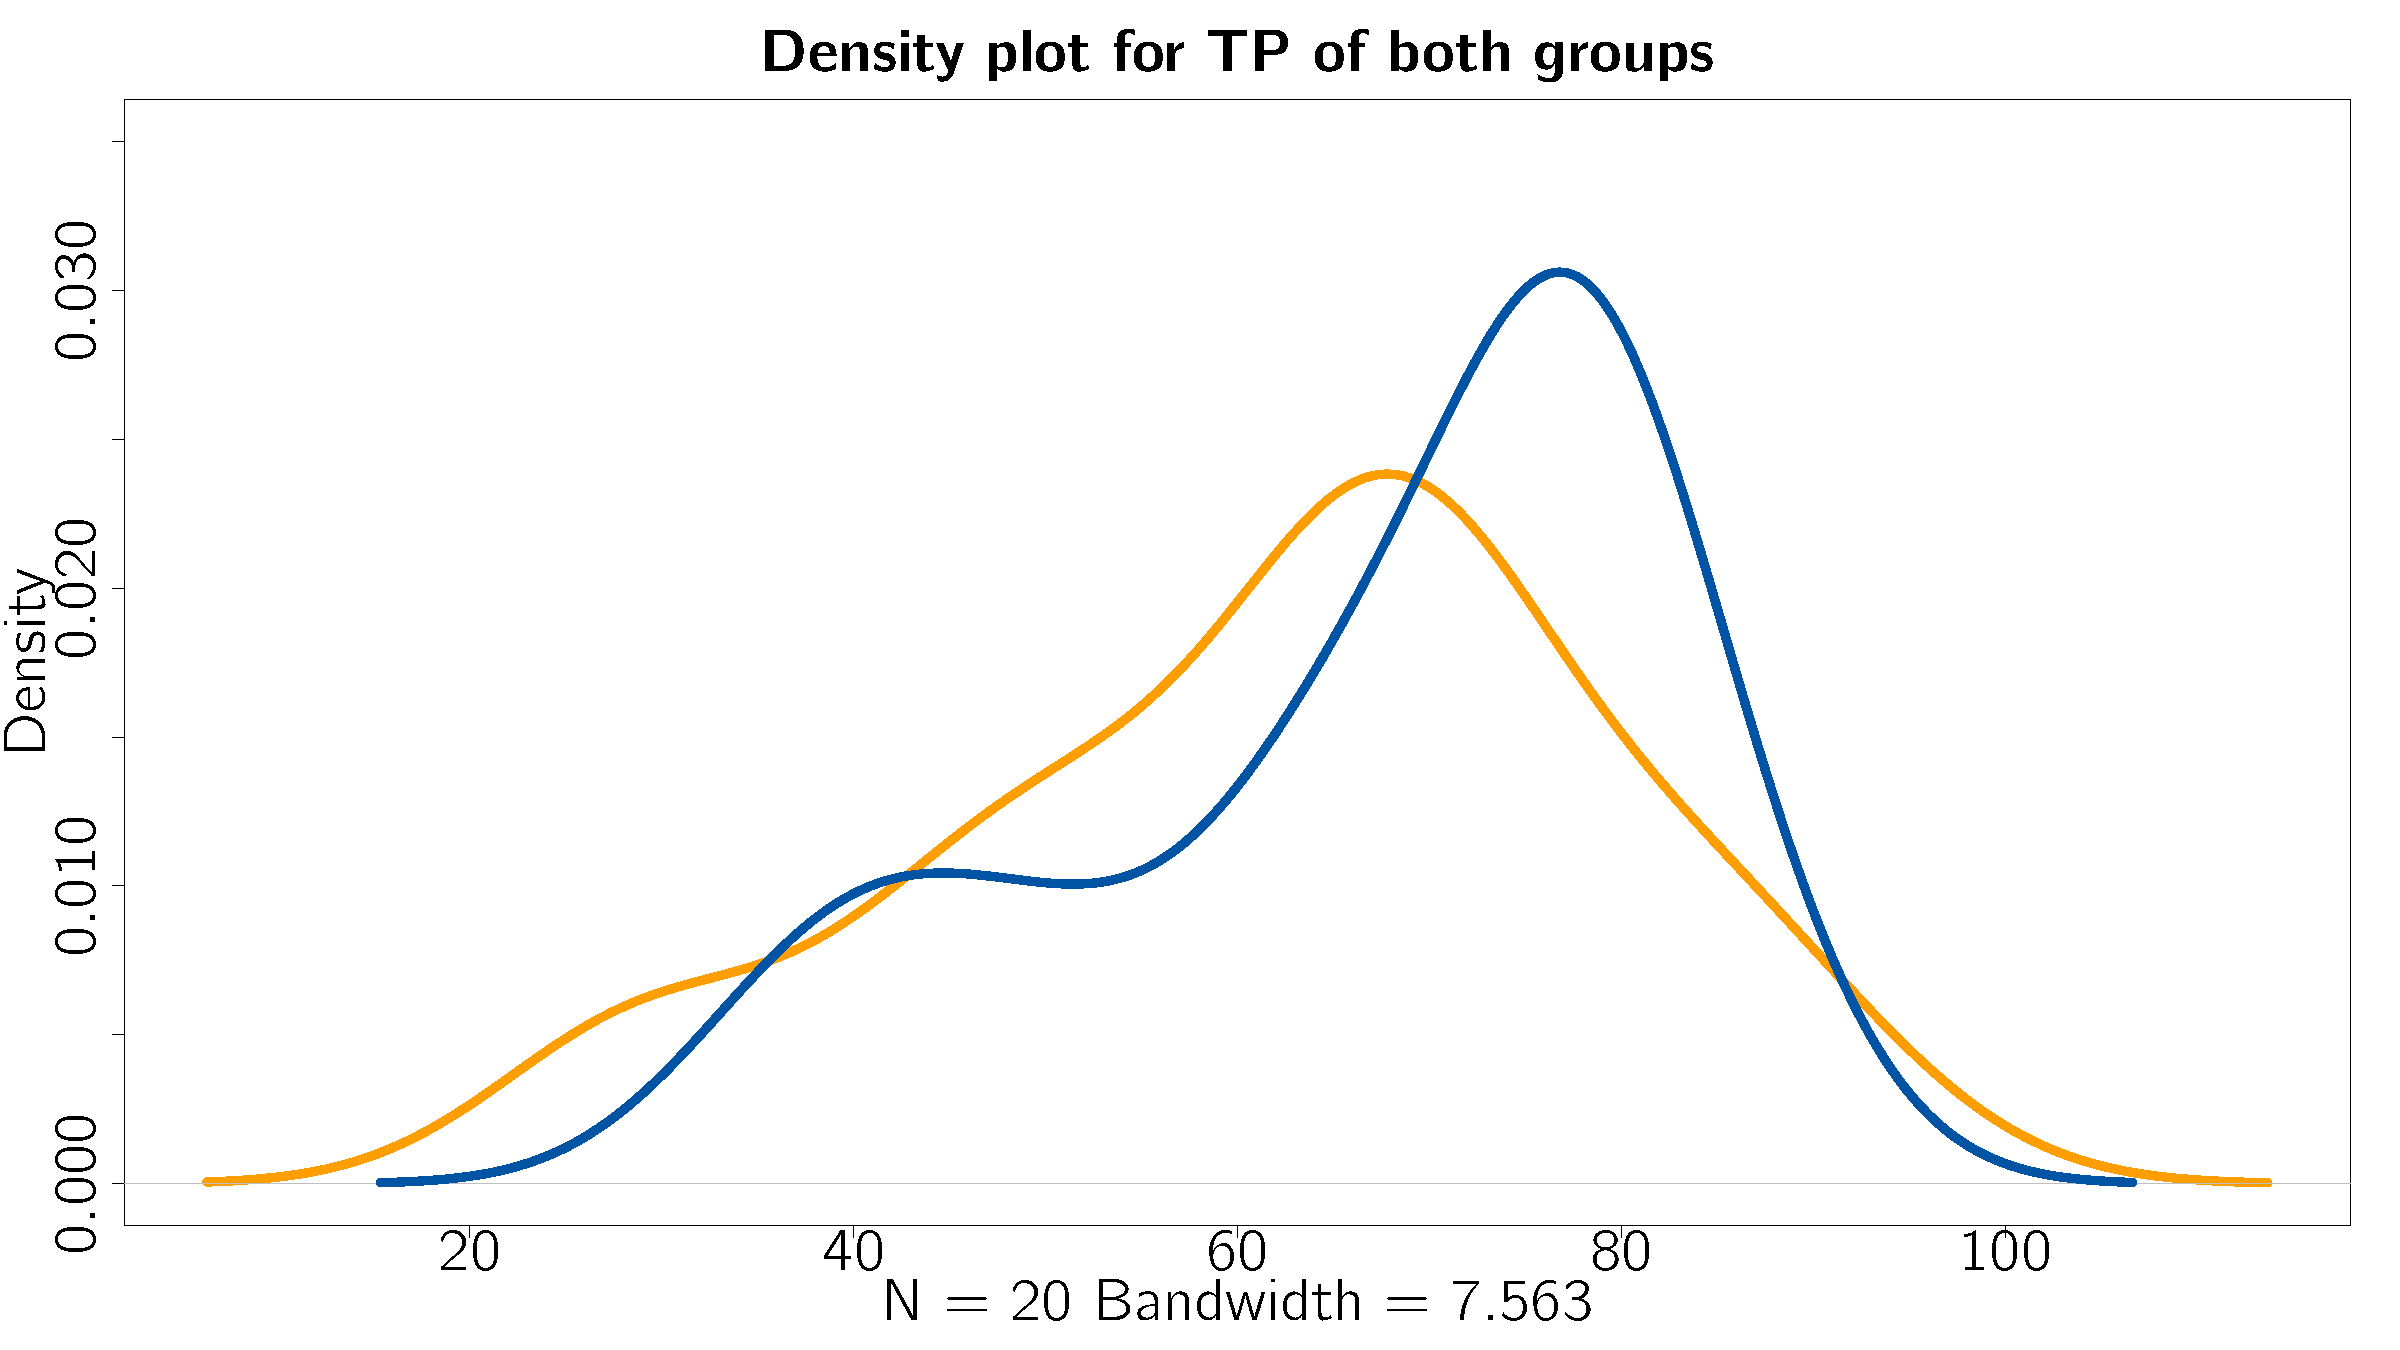
\includegraphics[width=.60\linewidth]{figure/beamer-density} 

}

\caption[Density plot for TP of both groups]{Density plot for TP of both groups\label{fig:density}}
\end{figure}


\end{knitrout}











\paragraph{Descriptive statistics}
Figure \ref{fig:gender} shows the gender distribution of the two samples. Figure \ref{fig:jobaffect} shows the emotion states of both groups during the d2 test according to the self-reported job-affect scale, whereas figure \ref{fig:emotions} shows the emotions experienced while watching the movie, which were surveyed using the post-film questionnaire. As the d2 test consisted of 14 sequences the completion rate per sequence is shown in figure \ref{fig:completed_sets}. In order to compare the performance of both groups the arithmetic mean for each group was calculated and used as the main measure for TP. Table \ref{moments_dist} provides an overview of the moments of distribution of TP. Figure \ref{fig:boxplots1} shows the performance in the d2 test, which represents the TP in this study with the support of boxplots, whereas figure \ref{fig:boxplots2} shows the accuracy of both groups in the d2 test. In the following paragraph the two groups are checked for significant differences with regard to TP.


%%%%%%%%%%%%%%%%%%%%%%%%%%%%%%%%%%%%
%%%%%%%  STATISTICS  %%%%%%%%%%%%%%%
%%%%%%%%%%%%%%%%%%%%%%%%%%%%%%%%%%%%
\begin{knitrout}\footnotesize
\definecolor{shadecolor}{rgb}{0.969, 0.969, 0.969}\color{fgcolor}\begin{figure}[]


{\centering 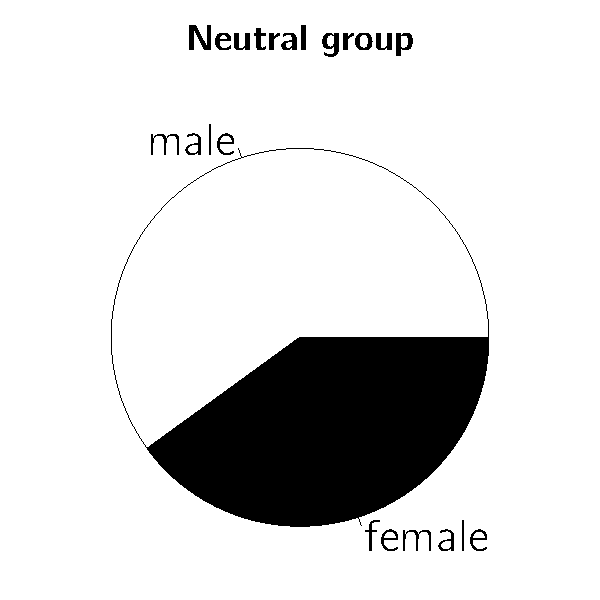
\includegraphics[width=.3\linewidth]{figure/beamer-gender1} 
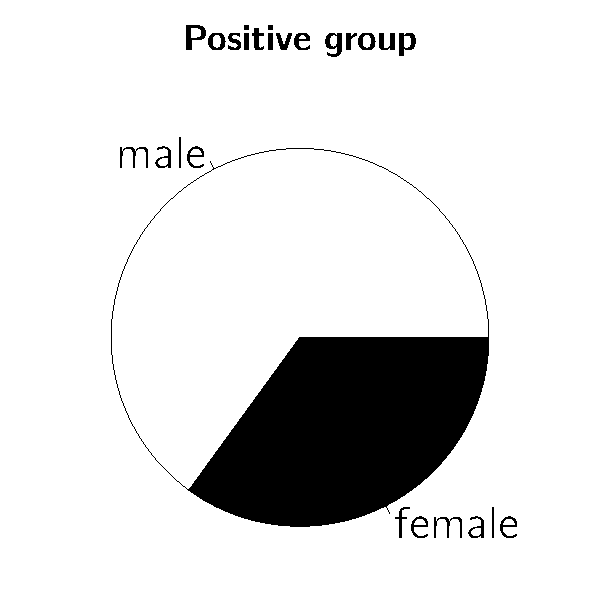
\includegraphics[width=.3\linewidth]{figure/beamer-gender2} 

}

\caption[Gender distribution]{Gender distribution\label{fig:gender}}
\end{figure}


\end{knitrout}





\begin{knitrout}\footnotesize
\definecolor{shadecolor}{rgb}{0.969, 0.969, 0.969}\color{fgcolor}\begin{figure}[]


{\centering 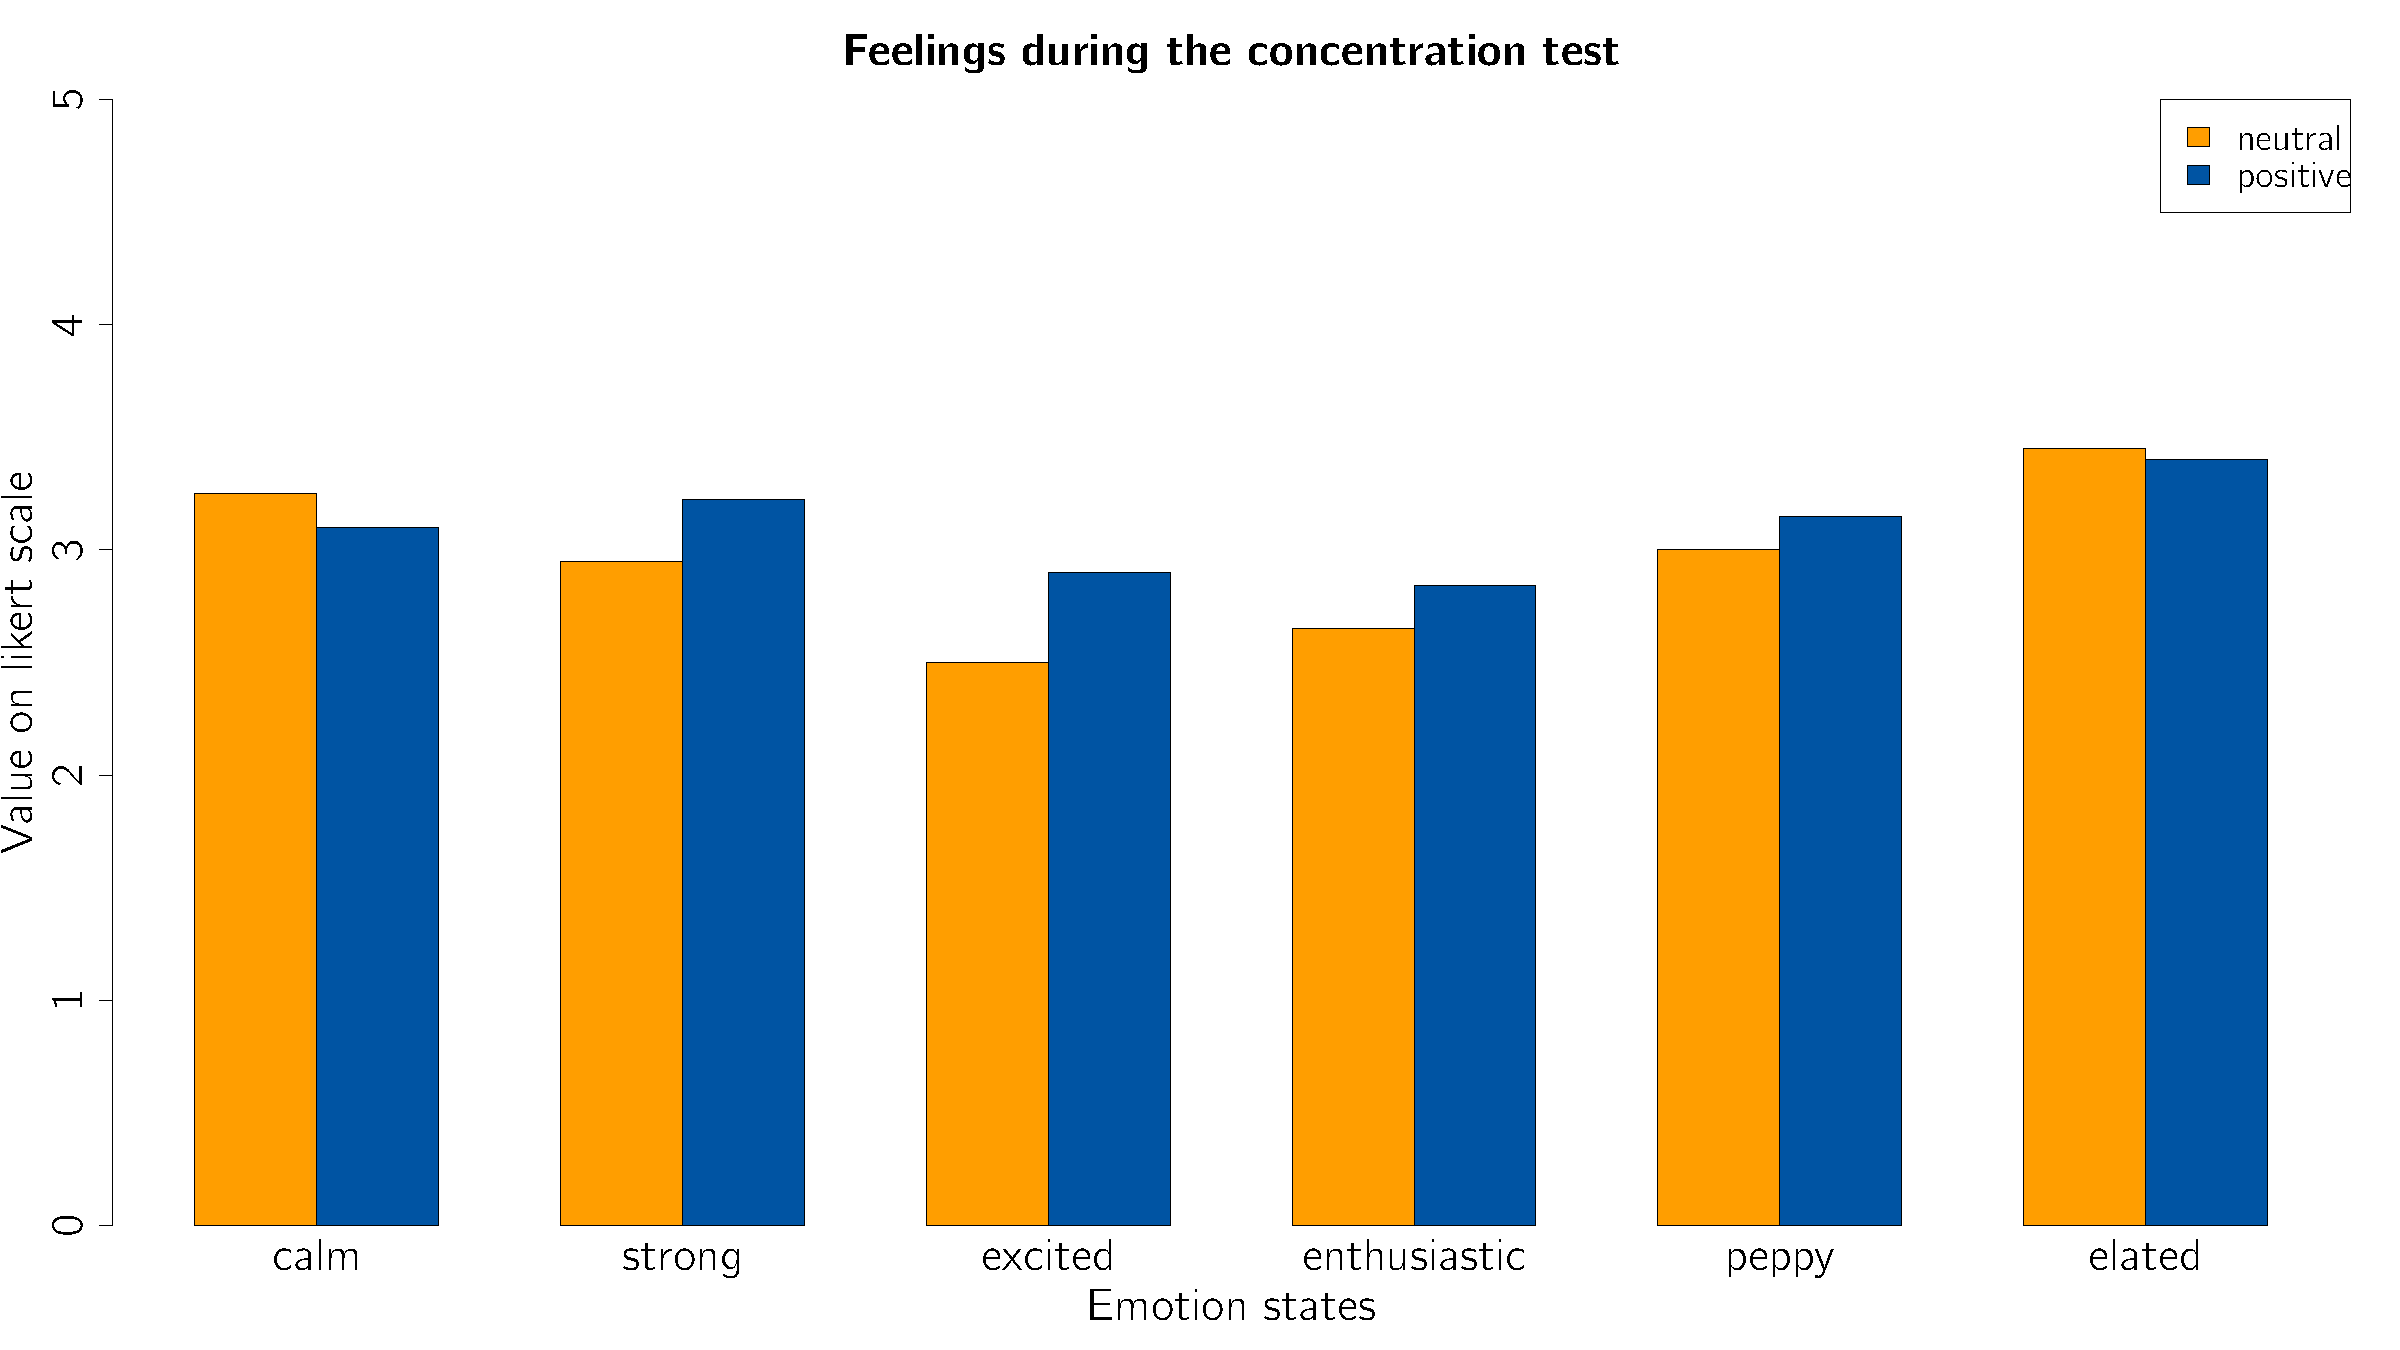
\includegraphics[width=1\linewidth]{figure/beamer-jobaffect} 

}

\caption[Results from the job affective scale (1=not at all]{Results from the job affective scale (1=not at all; 5=very much)\label{fig:jobaffect}}
\end{figure}


\end{knitrout}


\begin{knitrout}\footnotesize
\definecolor{shadecolor}{rgb}{0.969, 0.969, 0.969}\color{fgcolor}\begin{figure}[]


{\centering 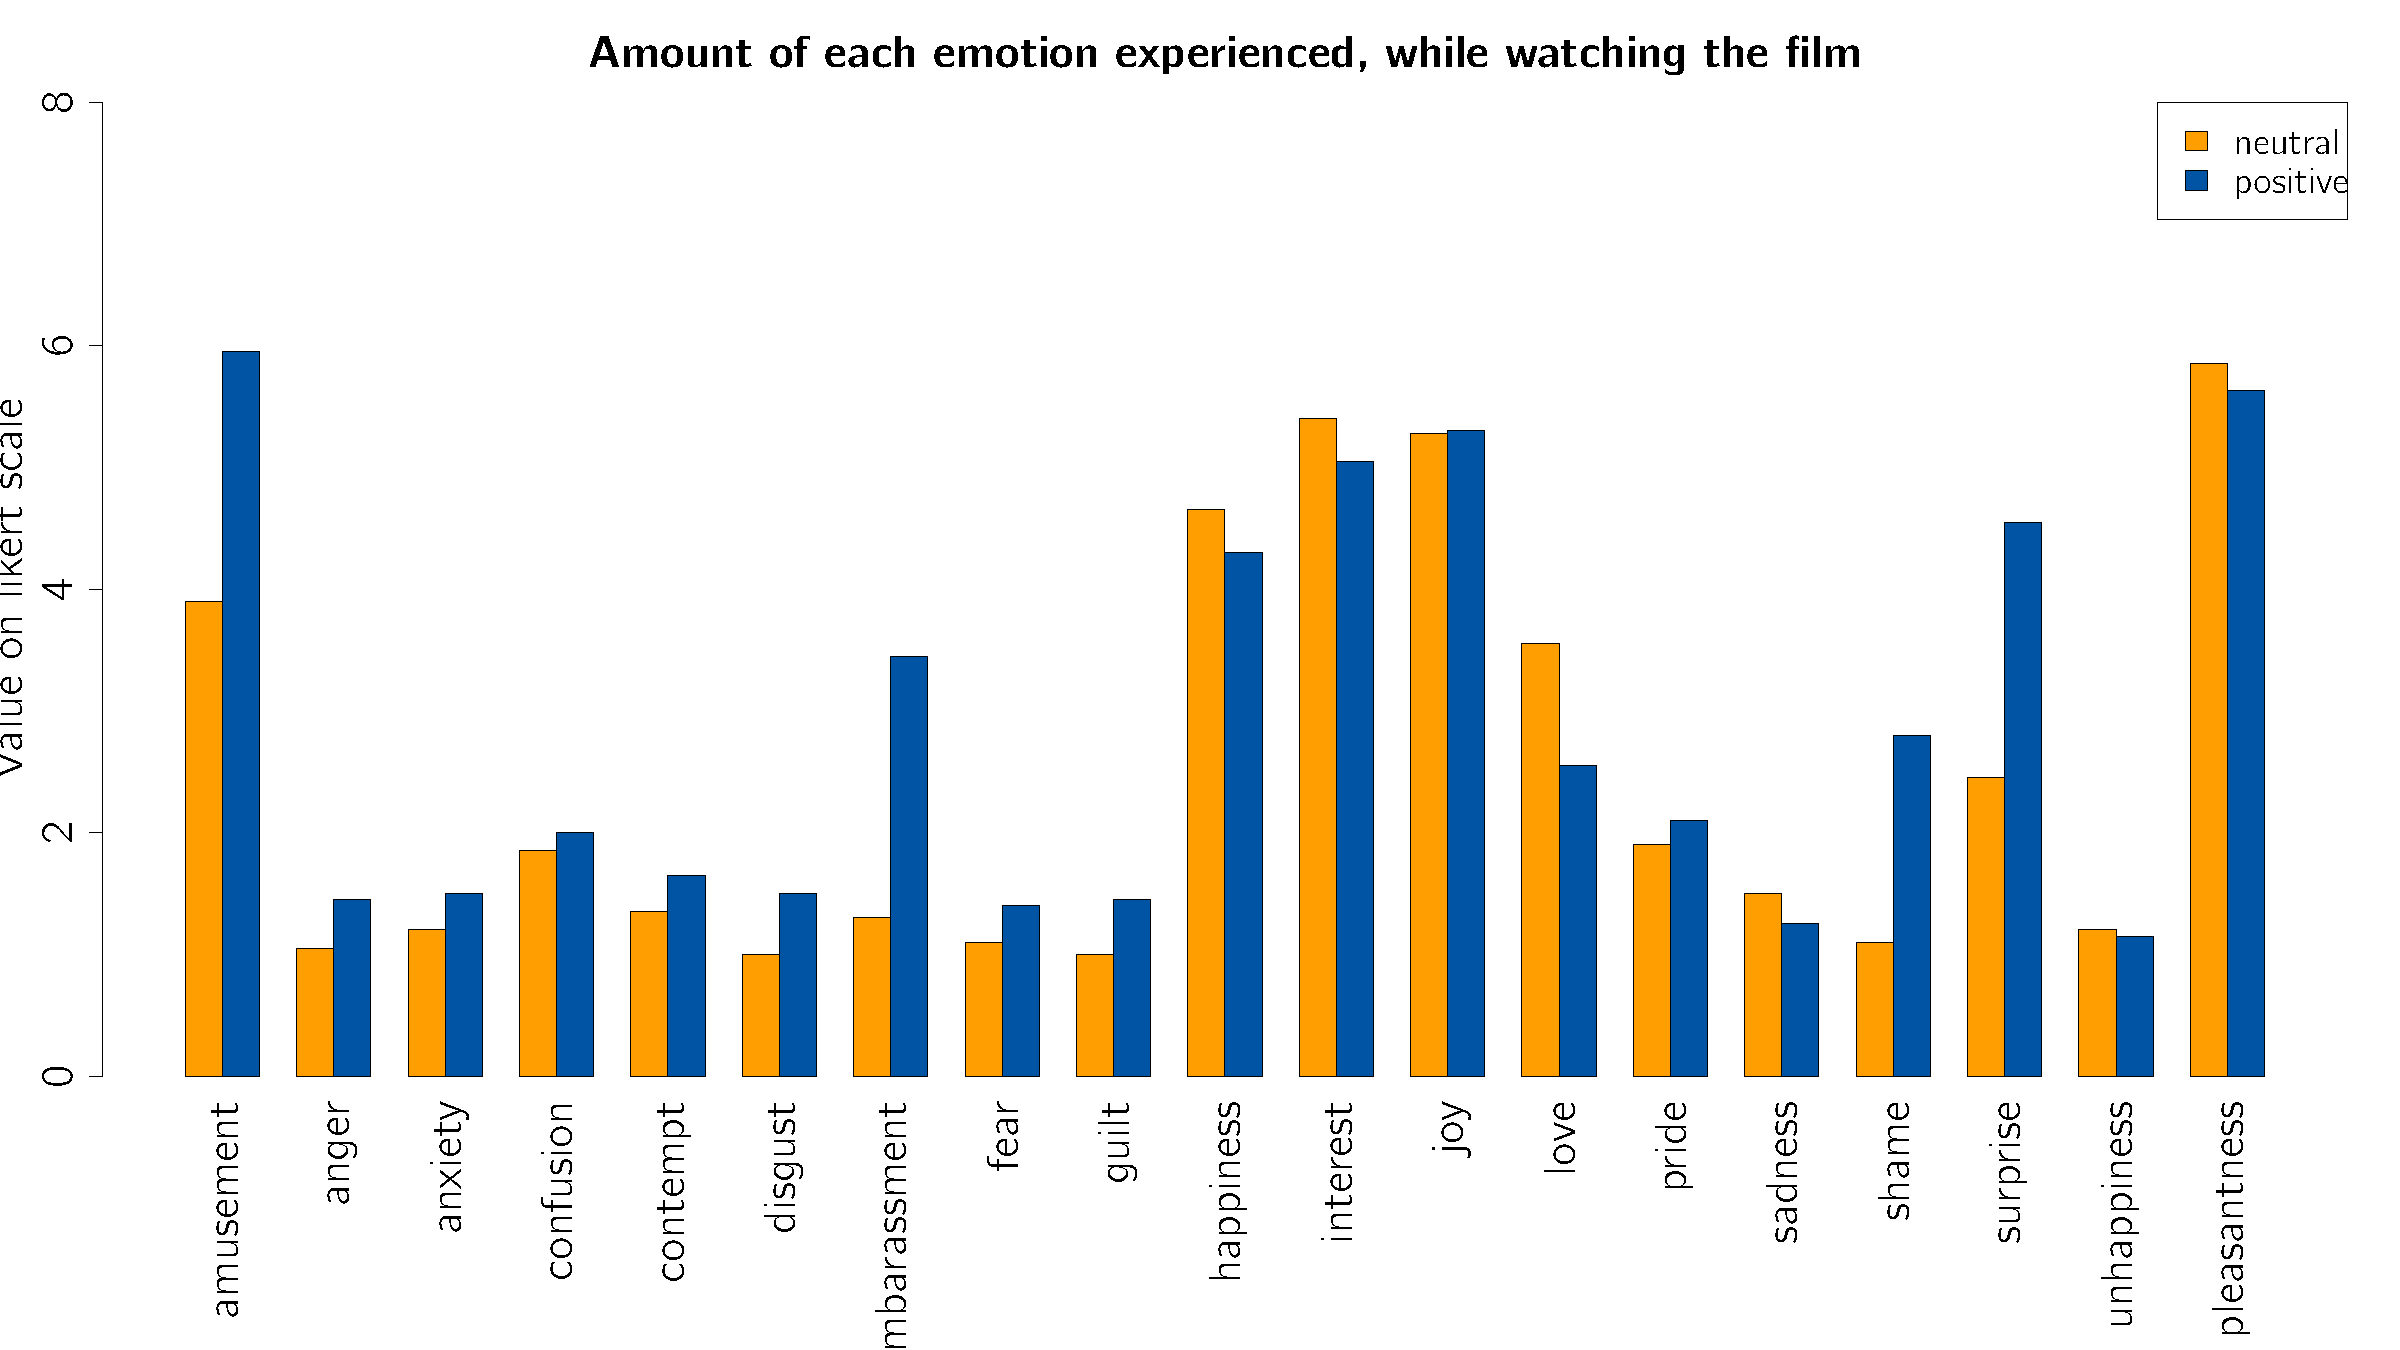
\includegraphics[width=1\linewidth]{figure/beamer-emotions} 

}

\caption[Emotions experienced while watching the film (1=none]{Emotions experienced while watching the film (1=none; 8=extremely)\label{fig:emotions}}
\end{figure}


\end{knitrout}





\begin{knitrout}\footnotesize
\definecolor{shadecolor}{rgb}{0.969, 0.969, 0.969}\color{fgcolor}\begin{figure}[]


{\centering 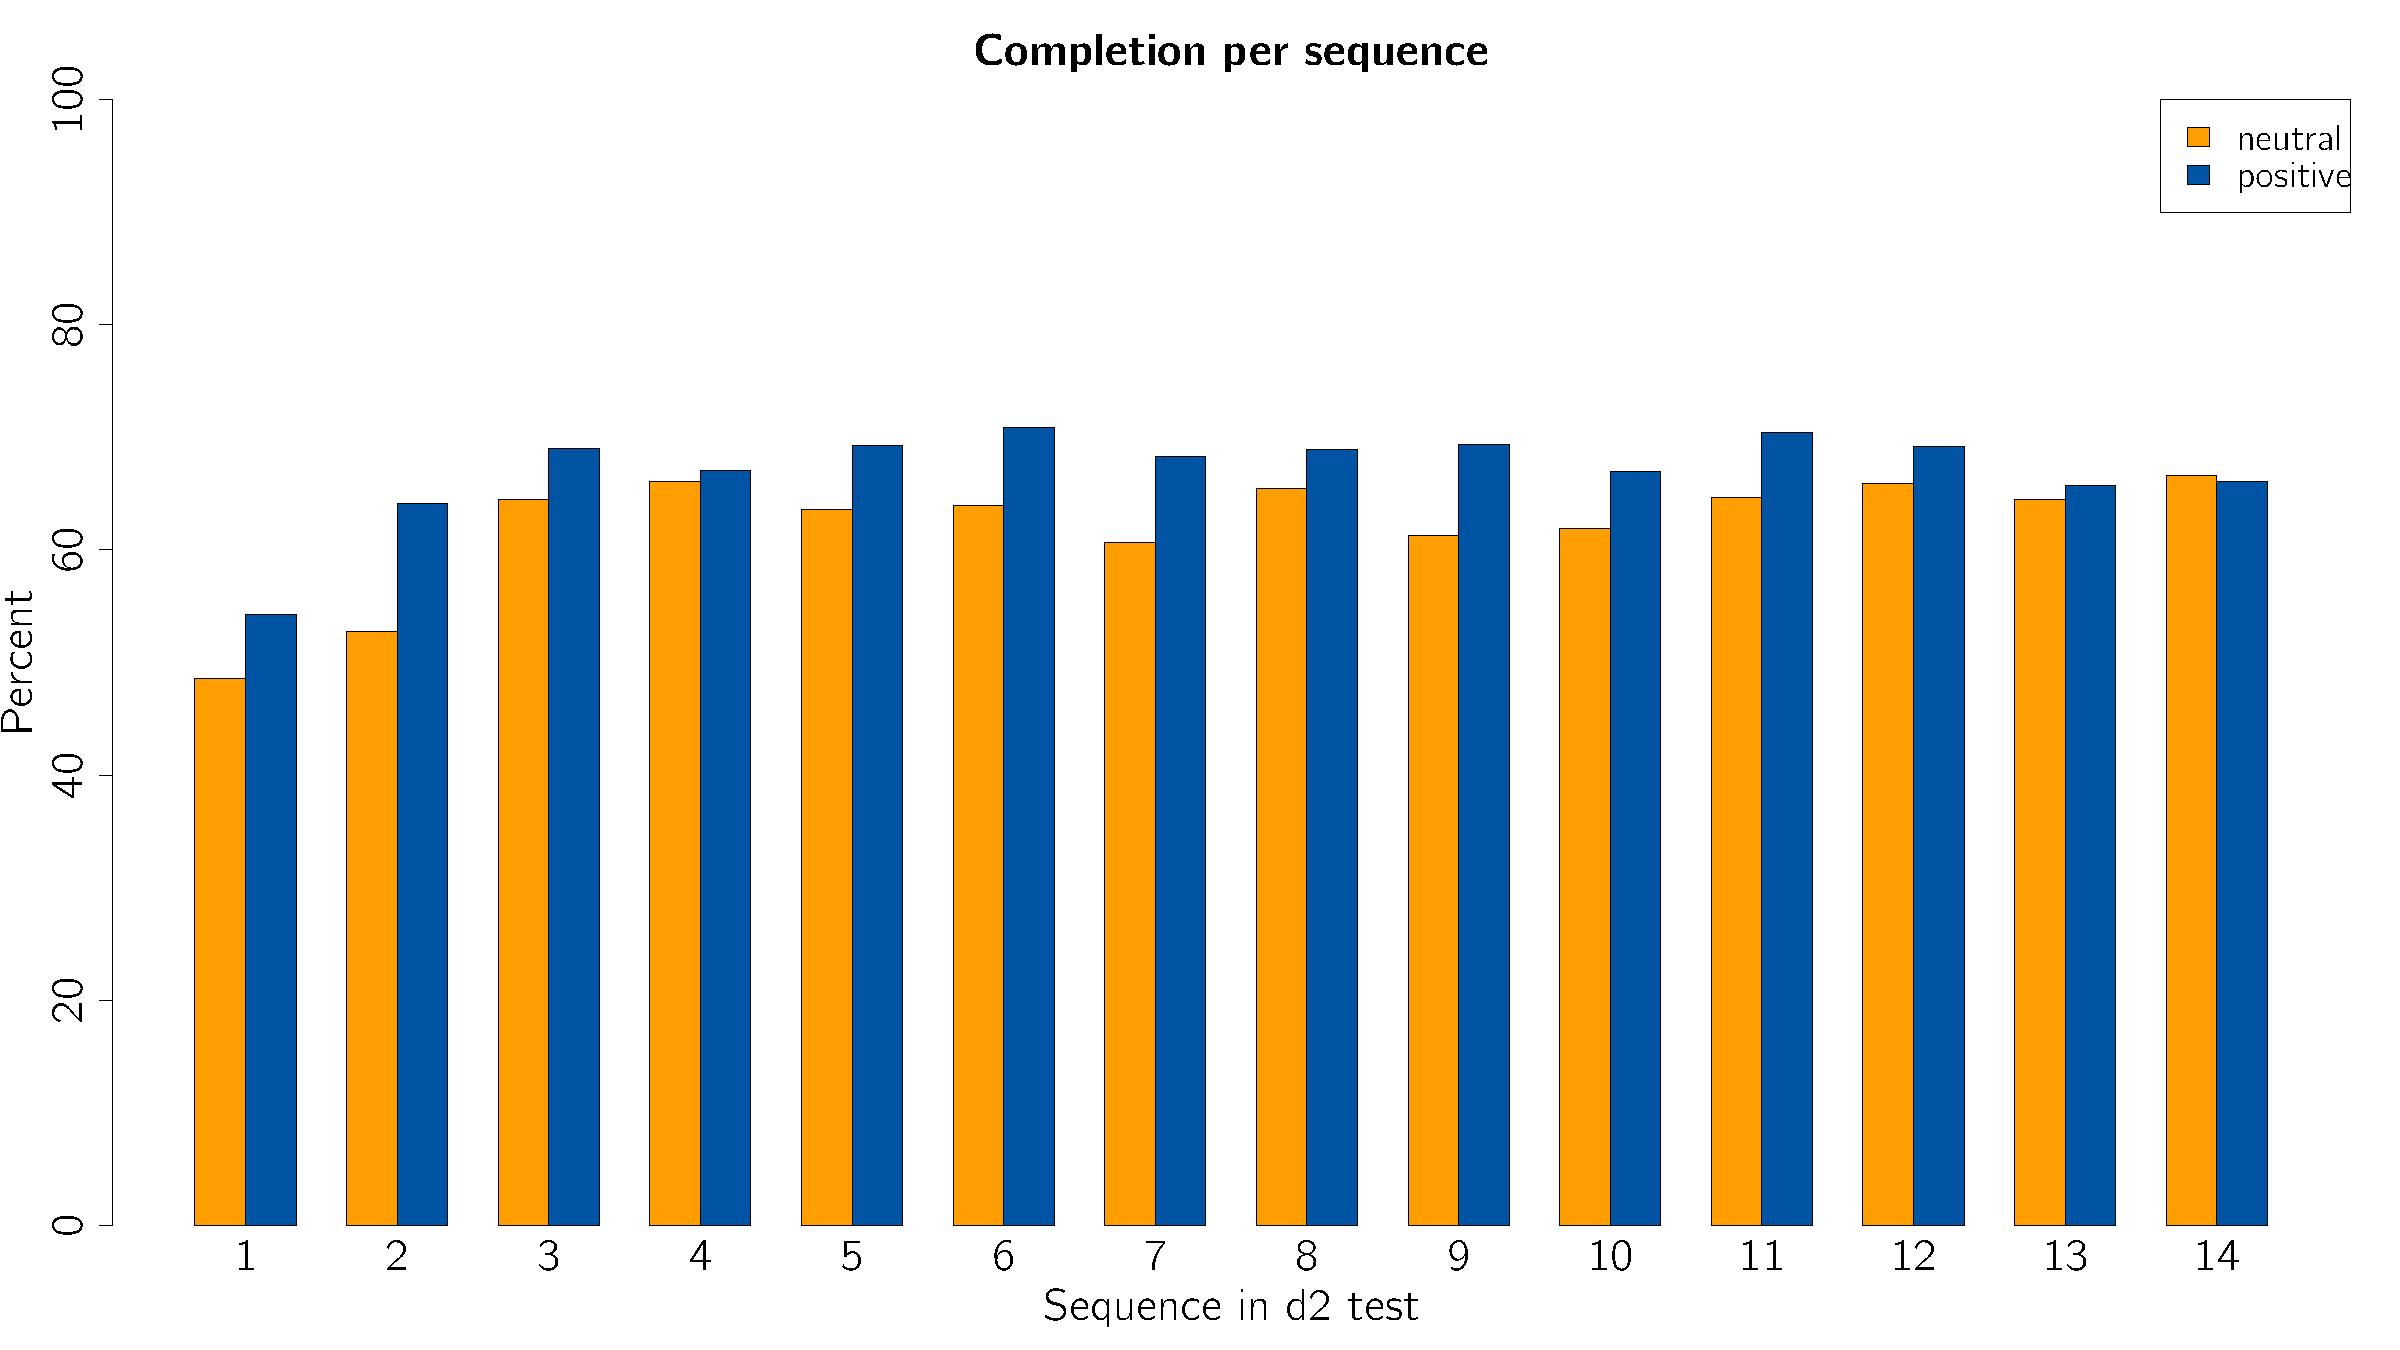
\includegraphics[width=1\linewidth]{figure/beamer-completed_sets} 

}

\caption[Performance over time]{Performance over time\label{fig:completed_sets}}
\end{figure}


\end{knitrout}


\begin{knitrout}\footnotesize
\definecolor{shadecolor}{rgb}{0.969, 0.969, 0.969}\color{fgcolor}\begin{figure}[]
\subfloat[Performance in d2 test\label{fig:boxplots1}]{

{\centering 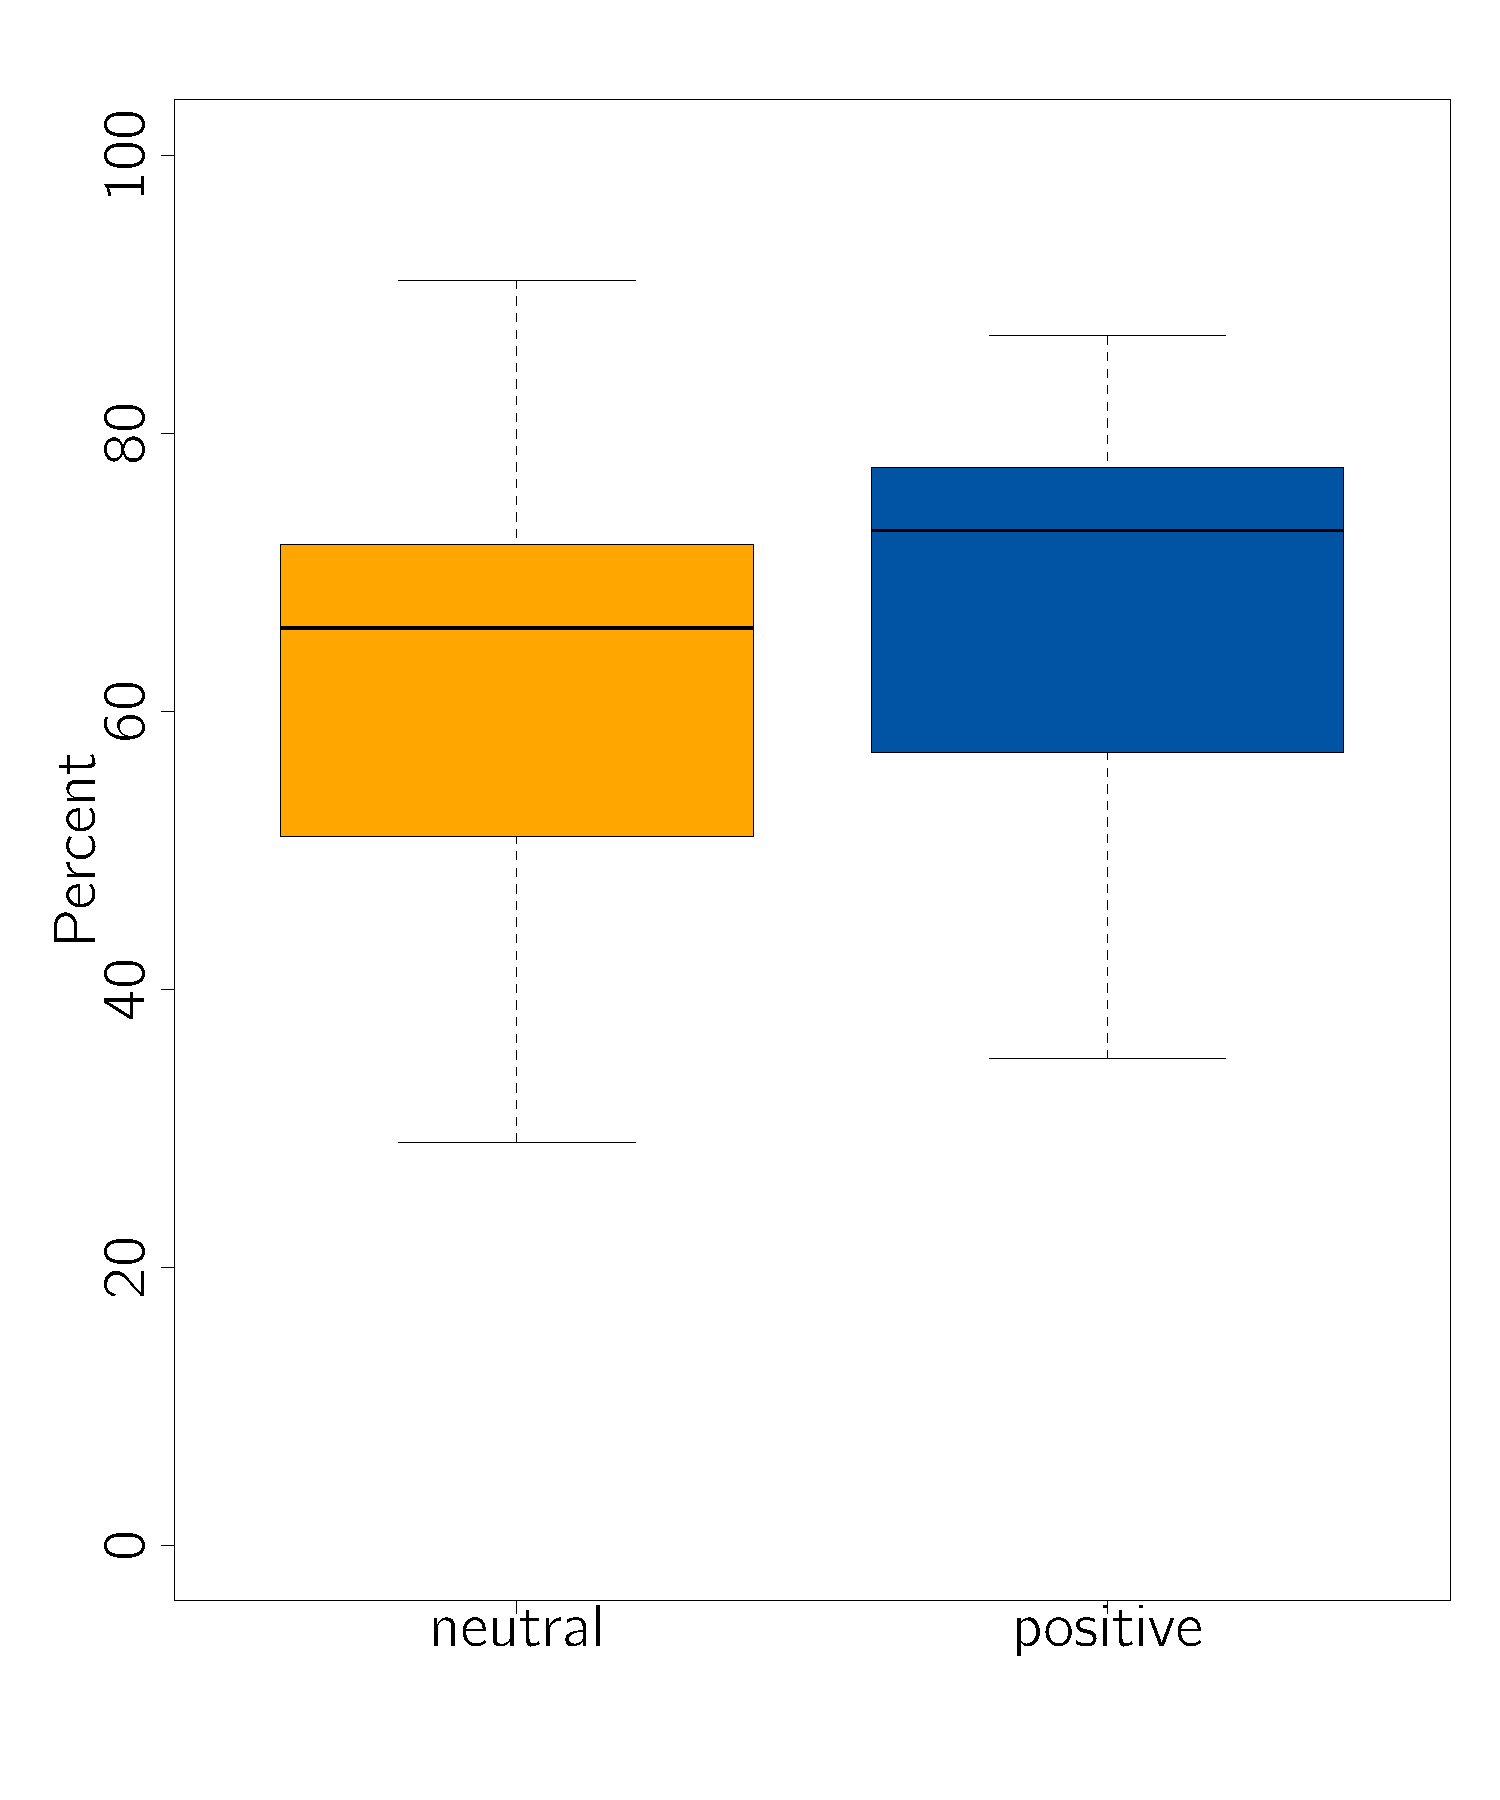
\includegraphics[width=.49\linewidth]{figure/beamer-boxplots1} 

}

}
\subfloat[Accuracy in d2 test\label{fig:boxplots2}]{

{\centering 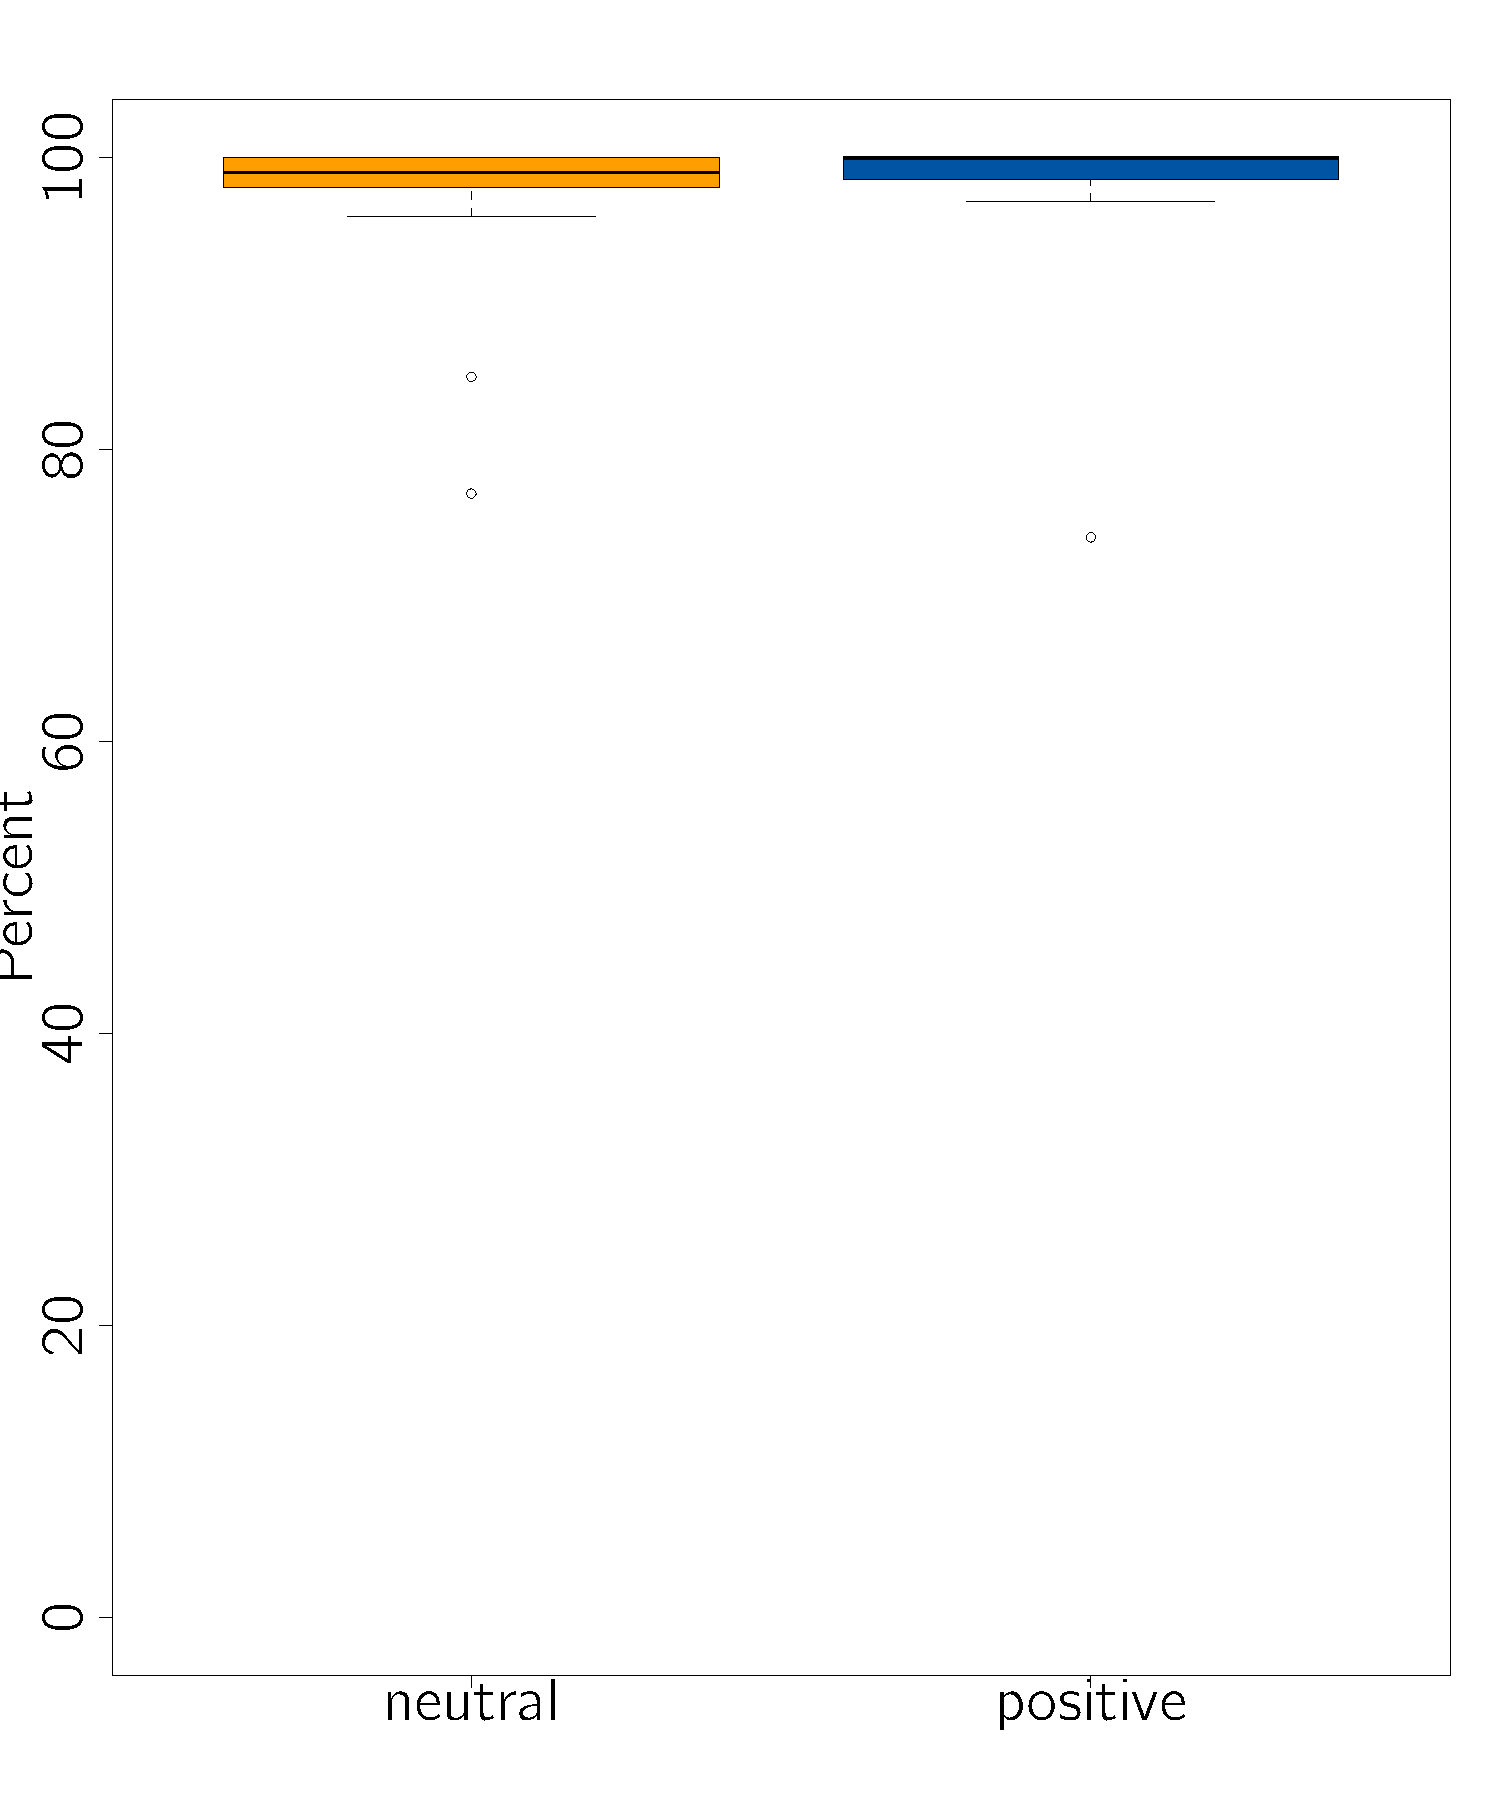
\includegraphics[width=.49\linewidth]{figure/beamer-boxplots2} 

}

}\caption[Comparison of sample means of d2 test results]{Comparison of sample means of d2 test results\label{fig:boxplots}}
\end{figure}


\end{knitrout}





\begin{table}[htb]
\caption{Moments of the distribution}
\centering
\begin{tabularx}{\textwidth}{XXX}
\toprule
  & neutral group & positive group\\ 
\midrule
\(\mu\) & 62.3 & 67.05 \\ 
\(\sigma^{2}\) & 297.27 & 237.21 \\ 
\(\sigma\) & 17.24 & 15.4 \\ 
\bottomrule
\end{tabularx} 
\label{moments_dist}

\end{table}













\paragraph{Independent two sample t-test}
\label{wilcoxon}
The independent two sample t-test was conducted to compare TP in neutral emotion conditions and positive emotion conditions. Although the t-test only can be applied for normal distributed data, a requirement, which is not fully fulfilled in the research paper at hand, the test was chosen as it is assumed, a bigger sample size would have lead to a normal distributed dataset \cite{Dalgaard2008}. The results show, there was not a significant difference in the scores for TP between neutral emotion conditions (\textit{M=}62.3, \textit{SD=}17.24) and positive emotion conditions (\textit{M=}67.05, \textit{SD=}15.4); \textit{t}(37.53)=-.92, \textit{p=}.18. In other words, watching a video, which should elicit positive emotions, does not have a significant influence on the performance in the d2 test compared watching a video which should elicit neutral emotions.

%The Mann-Whitney-Wilcoxon Test indicated that TP for participants who were shown a movie to elicit positive emotions (\textit{Mdn=}median(TP_pos)) was not significantly greater than for participants who were shown a movie with the aim to elicit neutral emotions (\textit{Mdn=}median(TP_neut)), \textit{U=}, \textit{p=}.17, \textit{r=}.\todo{check for values. is it the right test??}

%For the t-test use following references \cite{Dalgaard2008}. From the t-test results following expressions are derived: \(H_0: \mu_{neut}-\mu_{pos}=0\)\\ \(H_1: \mu_{neut}-\mu_{pos}<0\)\\As the difference between the means \(\mu_{neut}\) and \(\mu_{pos}\) are not significant, \(H_0\) can not be rejected and \(H_1\) can not be supported.



\section*{Discussion}
\paragraph{Limitations}
 %After seeing the results, the study raised several limitations that need to be discussed. One of the main limitations is the small sample size. GPower estimated a sample size of N = 70, but in the end, the experiments were only conducted with 40 participants. Another limitation might be that most of the participants were cohort students. Since  they heard about the project in class before, results might have been falsified due to knowledge about the work. Furthermore, the fact that a convenient sampling has been used - the majority of people were students from the GSU - leads to the assumption that the participants share similar characteristics to a certain extent. Another limitation can be the unstandardized setting. This means that not all of the experiments took place in the same setting, which was mainly due to access reasons. Since a lot of experiments took place in the library, noise might have been a distraction issue for participants. Limitations can also be seen in the choice of videos. The film for eliciting neutral emotions was not a scientific validated video. Comments of participants and the class discussion showed that this clip triggered rather positive emotions, due to the fact that a tropic beach area was shown during a more depressing and rainy real life climate. Even though the film used to elicit positive emotions was a scientific validated video, the fact that most participants were watching this scene in a crowded setting, might have given them a feeling of unpleasantness. There was no question that the clip put a smile on the participants face, but possibly the feeling of being watched might have restricted a positive state of mind.




After seeing what the outcomes of the study are, and the fact that the results were not significant, it is important to analyze the limitations that the project had to face. One of the main limitations is clearly the small sample size. As stated before, GPower estimated an N of 70. The group that has been worked with, was only about half of the needed size. This was mainly due to time issues, since the time frame of completing all of the experiments was fairly short and the research group was only able to conduct so many experiments. 
It should be added that more than half of the participants were cohort students. Since every group introduced their topic beforehand in class, some students might have, intentionally or not, remembered what the study was about and what the group was looking for and by this influenced their behavior during the experiment. 
Furthermore, the fact that a convenient sampling has been used, leads to the assumption that the participants somewhat had similar characteristics. The majority of people were students from the GSU. Again, the fact that a lot of participants were cohort students, supports this view, that the group of participants was not chosen completely random and might have had similar characteristics that have an impact on how the experiments were conducted.
Another aspect that might have had an impact on the outcome of the study was the condition of an unstandardised setting. This means that not all of the experiments took place in the same setting. This was mainly due to access reasons. Since the chosen laboratory was not available all the time, the main place for conducting the experiments was the library. Multiple influences, like noise and the movement of other students, must be taken into account here. 
Limitations can also be seen in the choice of videos. The movie that was chosen for eliciting neutral emotions has not been scientifically validated before. The research group took this video because of knowing that nature movies can have an influence on supporting a neutral state of mind. After talking to the participants and through the class discussion, it can be said that the “neutral” video tended to have more of a positive effect. While the real life climate was rather depressing and rainy, the presentation of a tropic beach area, gave the participants more of a warm feeling and therefore might have contributed to a rather positive state of mind. The positive movie might have also had a different effect than anticipated. Feedback of participants were that they sometimes did not feel too comfortable watching a scene where someone is feigning sexual excitement. Since this video has been used to elicit positive emotions in earlier experiments, it is more likely that the crowded setting triggered the feeling of being uncomfortable than the video itself.


\paragraph{Implications for further research}
In the end, the results are not showing the significant difference that the research group was hoping for. Thoughts on this were that the design and the research questions should have gone further than just measuring the difference between positive and neutral emotions. It is hard to say, if these two emotions might be too close to each other, especially in an experiment that only lasts for 15 minutes and where this certain state of mind needs to be triggered in the first place. One idea is to add a third experimental group, which would be dealing with a movie that is supposed to elicit negative emotions. In this case, at least on a first and obvious observation, the difference between the emotions would be greater than just between a positive and neutral state of mind. However, this option was not considered because of time reasons. Since the research group was only able to find 20 participants for each of the groups, including a third experimental group might have resulted in even less participants for each emotion and therefore in less significance in the results.


\section*{Conclusion}
Finalizing, even if the results were not significant, probably mainly based on the mentioned limitations, a tendency towards a better performance of the positive group could be observed. Additional research could contribute to the topic of how far PE have an influence on TP and link it to a wider theoretical framework. A better understanding of the influence of certain emotion states on human behaviour could contribute to optimize leadership in non-profit organizations and the behaviour of superiors accompanied by less vulnerability towards social conflicts and economic ineffectiveness. This knowledge is necessary, especially in times of decreasing volunteering rates amongst the German population.

%\newpage
%---------------------------------------------------------------------
% BIBLIOGRAPHY:
\bibliographystyle{apacite}
\renewcommand{\bibliographytypesize}{\small} % set font size for bibliography
\interlinepenalty 10000 % no pagebreaks within citations
%\bibliography{ref_leadership} % defines the *.bib-file where your references are in. File needs to have the ending *.bib
\bibliography{library}

\newpage
\appendix
%\pagenumbering{roman}
\section{Statistical Output and Questionnaire}
\subsection{Shapiro-Wilk Normality Test}



\begin{knitrout}\footnotesize
\definecolor{shadecolor}{rgb}{0.969, 0.969, 0.969}\color{fgcolor}\begin{kframe}
\begin{alltt}
\hlkwd{shapiro.test}\hlstd{(TP_neut)}
\end{alltt}
\begin{verbatim}
## 
## 	Shapiro-Wilk normality test
## 
## data:  TP_neut
## W = 0.9586, p-value = 0.5166
\end{verbatim}
\begin{alltt}
\hlkwd{shapiro.test}\hlstd{(TP_pos)}
\end{alltt}
\begin{verbatim}
## 
## 	Shapiro-Wilk normality test
## 
## data:  TP_pos
## W = 0.8935, p-value = 0.03124
\end{verbatim}
\end{kframe}
\end{knitrout}


\subsection{Independent two sample t-test}






\begin{knitrout}\footnotesize
\definecolor{shadecolor}{rgb}{0.969, 0.969, 0.969}\color{fgcolor}\begin{kframe}
\begin{alltt}
\hlkwd{t.test}\hlstd{(TP_neut, TP_pos,} \hlkwc{alternative} \hlstd{=} \hlstr{"less"}\hlstd{)}
\end{alltt}
\begin{verbatim}
## 
## 	Welch Two Sample t-test
## 
## data:  TP_neut and TP_pos
## t = -0.9188, df = 37.53, p-value = 0.182
## alternative hypothesis: true difference in means is less than 0
## 95 percent confidence interval:
##   -Inf 3.968
## sample estimates:
## mean of x mean of y 
##     62.30     67.05
\end{verbatim}
\end{kframe}
\end{knitrout}

\subsection{Questionnaire}

%\begin{landscape}



\begin{figure}
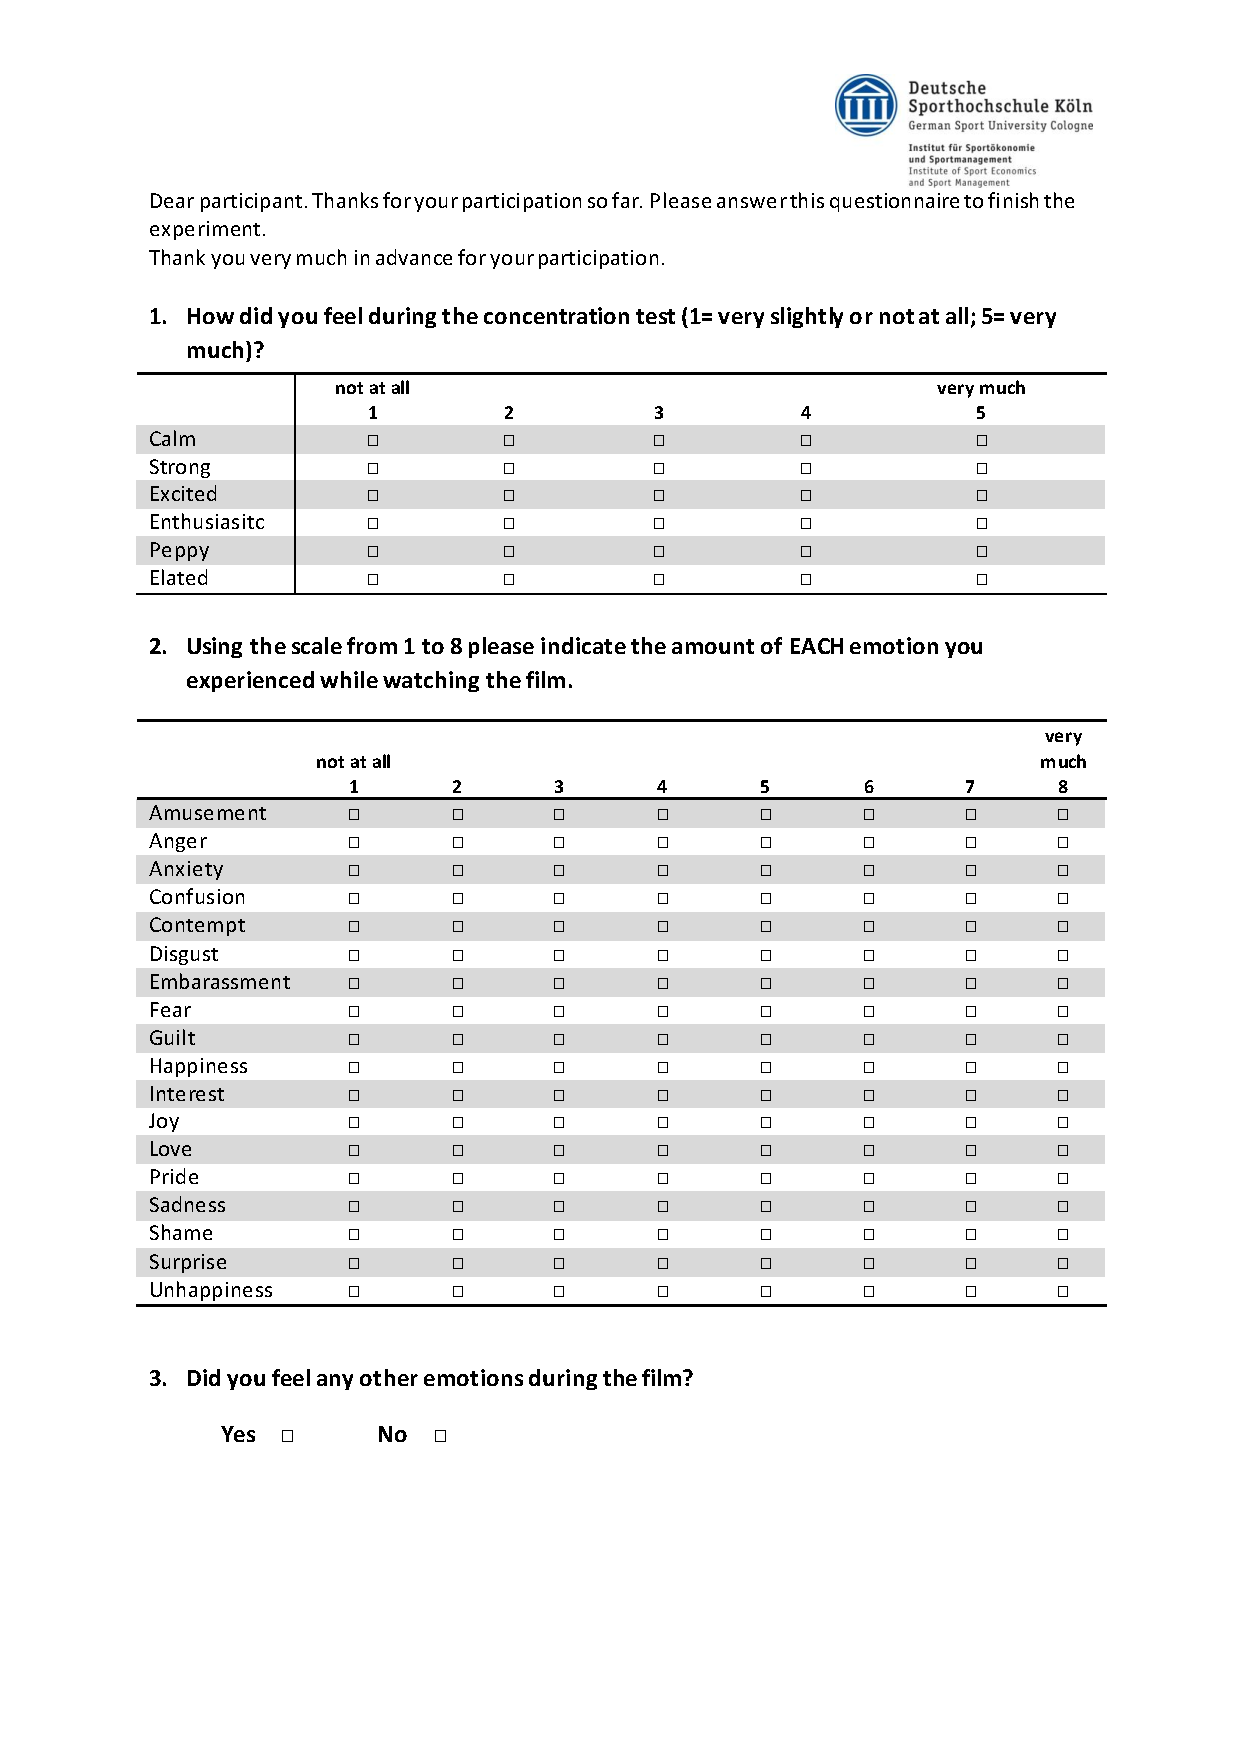
\includegraphics[width=0.75\textwidth, angle=90]{graphics/1_questionnaire_en.pdf}
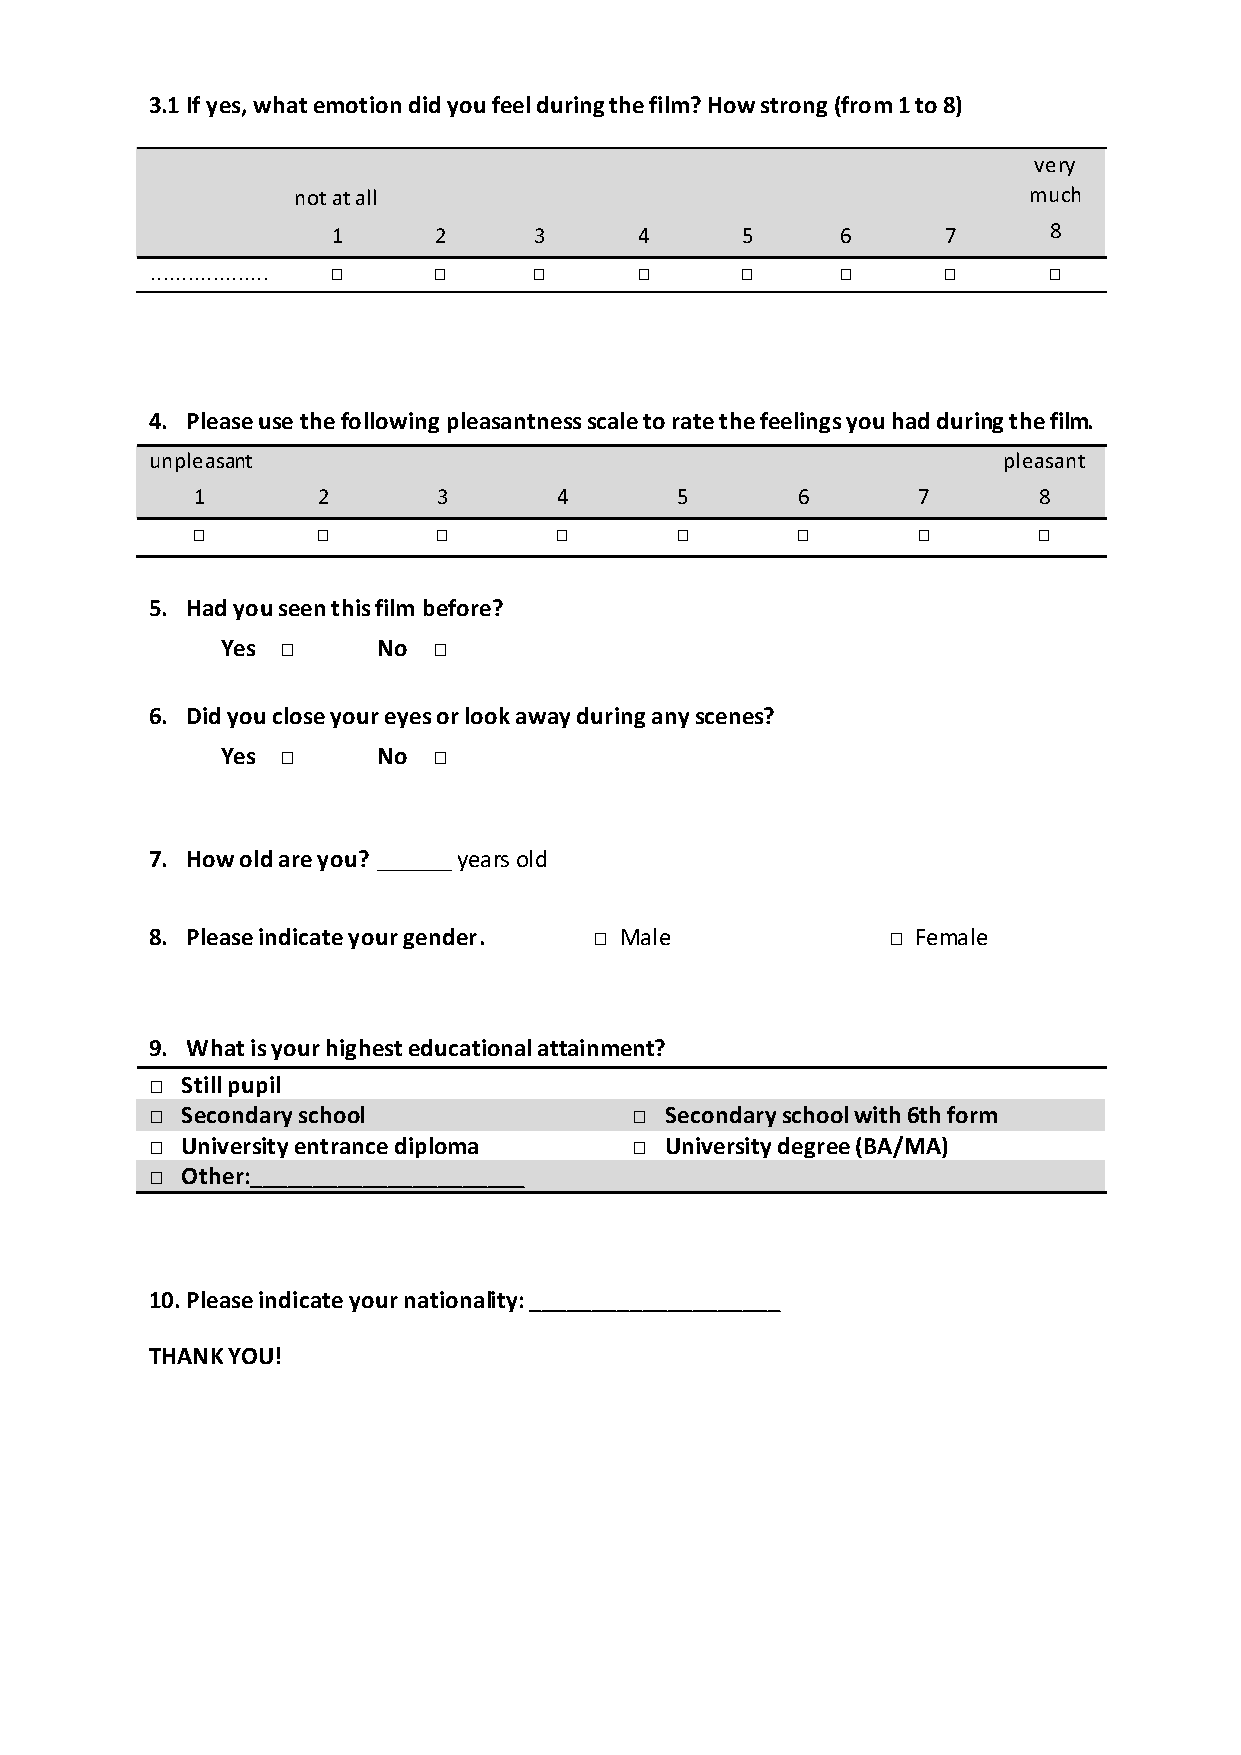
\includegraphics[width=0.75\textwidth, angle=90]{graphics/2_questionnaire_en.pdf}
\caption{The questionnaire used for the experiment}
\end{figure}
%\end{landscape}

\newpage



\end{document}
